\documentclass[11pt]{article}

\usepackage[margin=1in]{geometry}
\usepackage{amsmath,amssymb,amsthm}
\usepackage{graphicx}
\usepackage{booktabs}
\usepackage{multirow}
\usepackage{natbib}
\usepackage[ruled,vlined]{algorithm2e}
\usepackage{float}
\usepackage{tikz}
\usetikzlibrary{positioning,fit,arrows.meta,backgrounds,calc}
\usepackage[colorlinks=true,linkcolor=blue,citecolor=blue,urlcolor=blue]{hyperref}
\usepackage{microtype}
\usepackage{xcolor}

\newcommand{\shortclosepct}{97\%}
\newcommand{\truncgapmax}{1.38}
\newcommand{\klreduxfactor}{44.2$\times$}
\newcommand{\beyondgain}{0.024}
\newcommand{\beyondheadroom}{0.061}
\newcommand{\beyondgainpct}{39\%}
\newcommand{\certmarginmin}{0.03}
\newcommand{\certmarginmax}{1.30}
\newcommand{\chunkonekl}{0.019}
\newcommand{\chunkfivekl}{0.283}


\newcommand{\Dtot}{D_{\mathrm{tot}}}
\newcommand{\Dfar}{D'}
\newcommand{\Dloc}{D}
\newcommand{\KL}[2]{\mathrm{KL}\!\left(#1 \,\middle\|\, #2\right)}
\newcommand{\rep}{\mathrm{rep}}
\newtheorem{proposition}{Proposition}
\newtheorem{remark}{Remark}
\newcommand{\cmark}{\ding{51}}
\newcommand{\xmark}{\ding{55}}
\usepackage{pifont}

\title{\textbf{LongRange-PFN: KL-Distilled Recursive Latent Summaries\\
for Prior-Fitted Networks beyond the Context Window}}

\author{%
\begin{tabular}{cc}
\textbf{Antonio J.\ Brych} & \textbf{Gabriel Abad}\\
FGV EMAp & FGV EMAp\\
\end{tabular}
}

\date{Preprint. \today}

\begin{document}
\maketitle

\begin{abstract}
Prior-fitted networks (PFNs) predict a Bayesian posterior in one forward
pass, but only up to the context size seen in training: attention is
quadratic, and quality degrades past that window. LongRange-PFN compresses
a distant part of the context, $\Dfar$, into $k$ latent tokens
$z = \rep(\Dfar)$ with a learned summarizer, and predicts from the
remaining local context $\Dloc$ with $z$ added as extra tokens. A student
is distilled from a frozen, full-context teacher PFN by matching predictive
distributions; since both use the same discretized output, the KL between
them is exact. A recursive summarizer, $z_t = \rep(C_t, z_{t-1})$, folds
the distant context one chunk at a time and keeps constant state, so
inference is no longer capped by the training window. On Gaussian process
priors, where the true posterior is known, the student's NLL falls
\certmarginmin--\certmarginmax{} nats below a lower bound available to any
method that sees only $\Dloc$, closing \shortclosepct{} of the truncation
gap, and in a streaming setting with $4\times$ the training window the
recursive summary also beats a teacher restricted to the most recent
points, recovering $\approx\beyondgainpct{}$ of the remaining headroom.
Two things do not work yet: multi-chunk summarization stays noticeably
worse than single-shot even after fixing the model-selection criterion that
first hid it, consistent with error compounding across recursive steps;
and bounded-state inference still loses to classical full-context baselines
on this prior, where exact inference is cheap.
\end{abstract}

\section{Introduction}
\label{sec:intro}

Prior-fitted networks \citep{muller2022pfn} treat Bayesian prediction as
in-context learning: pre-train a transformer on data sets drawn from a
prior, then at test time feed it a training set $\Dtot$ and a query $x$ and
read off an approximation to $p(y \mid x, \Dtot)$. TabPFN
\citep{hollmann2023tabpfn, hollmann2025tabpfn} turned this into a working
tabular model, but the context is the model's memory: every observation is
a token, attention is quadratic, and the network has never seen contexts
larger than some $N$ during training. Past that size it is answering a
question it never practiced.

Three lines of work address this (Section~\ref{sec:related}): optimizing a
compact context per dataset at test time
\citep{feuer2024tunetables, ma2024icd}, retrieving real neighbors instead of
the whole context \citep{thomas2024localpfn}, and, in language models,
compressing prompts into soft tokens
\citep{mu2023gisting, ge2023icae, chevalier2023autocompressors}. None gives
a PFN a fixed-size, reusable summary of what the far-away data contributed
to the posterior.

LongRange-PFN splits $\Dtot = \Dfar \cup \Dloc$,
compresses $\Dfar$ into $k$ latent tokens $z = \rep(\Dfar)$ with a learned
summarizer (one forward pass, no test-time optimization), and predicts from
$[\,z \mid \Dloc \mid x\,]$ with a standard PFN backbone that treats $z$ as
ordinary context. Training distills a frozen, full-context teacher PFN:
teacher and student share the same discretized (``bar'') output, so the KL
between their predictions is an exact categorical KL with no sampling.

The summarizer is also recursive: $z_t = \rep(C_t, z_{t-1})$ folds a stream
of context chunks into a fixed-size summary, mirroring the Bayesian
filtering update $p(\rho \mid C_{1:t}) \propto p(C_t \mid \rho)\,
p(\rho \mid C_{1:t-1})$ over a latent task $\rho$. This decouples how much
data the system uses from the window any component was trained with:
distilled only on contexts up to $80$ points and $3$ chunks, at inference
the recursion handles $320$ points in five chunks, and beats a strong
recency baseline rather than just matching it (Table~\ref{tab:beyond}).

\paragraph{Contributions.}
\begin{enumerate}
  \item A summary-conditioned PFN trained by predictive KL distillation
  (Section~\ref{sec:method}): $\rep_\phi(\Dfar)$ is learned end-to-end so
  that $q_\phi(y \mid x, \Dloc, z)$ matches a frozen teacher's
  $p_\theta(y \mid x, \Dtot)$, with an exact bucket-level KL.
  \item A recursive summary update (Section~\ref{sec:recursive}) that gives
  bounded-state, anytime PFN inference beyond the pre-training window,
  to our knowledge the first such mechanism for PFNs. In our experiments it
  beats a recency baseline that gets to keep all its raw data, and we show
  where it still falls short.
  \item Validation against the exact posterior (Section~\ref{sec:experiments}):
  on GP priors we compare the whole pipeline to the true PPD, not just to
  the teacher, including a regime where the teacher cannot operate at all.
\end{enumerate}

\begin{figure}[t]
\centering
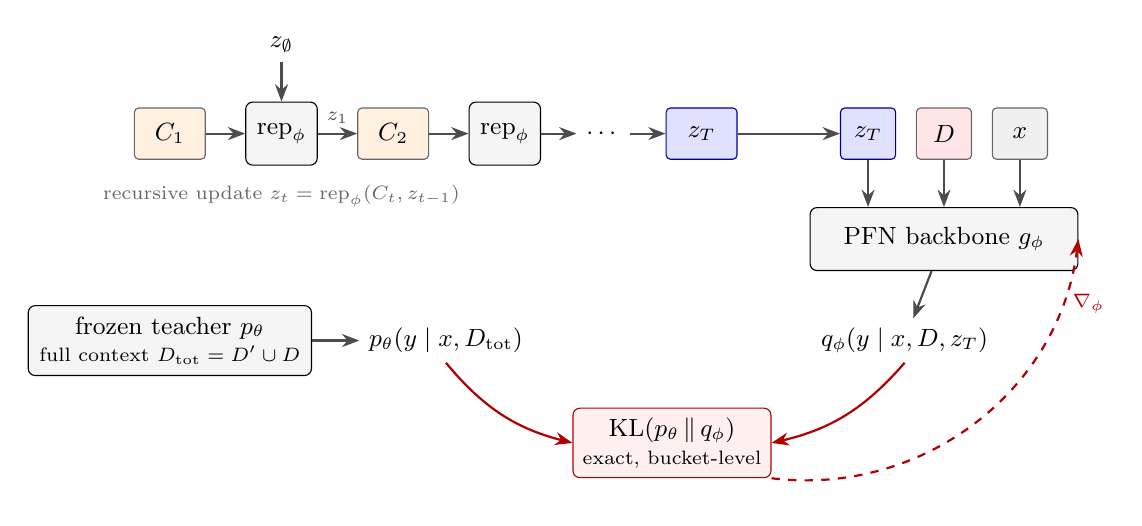
\begin{tikzpicture}[
  font=\small,
  chunk/.style={draw=black!60, fill=orange!12, rounded corners=1.5pt,
    minimum width=9mm, minimum height=6.5mm, inner sep=1.5pt},
  ztok/.style={draw=blue!60!black, fill=blue!12, rounded corners=1.5pt,
    minimum width=9mm, minimum height=6.5mm, inner sep=1.5pt},
  module/.style={draw=black, fill=black!4, rounded corners=2.5pt,
    minimum height=8mm, inner sep=4pt, align=center},
  loss/.style={draw=red!70!black, fill=red!6, rounded corners=2.5pt,
    minimum height=7mm, inner sep=3.5pt, align=center},
  arr/.style={-{Stealth[length=2.2mm]}, thick, black!70},
]
% streaming summarizer (left)
\node[chunk] (c1) {$C_1$};
\node[module, right=5mm of c1] (rep1) {$\rep_\phi$};
\node[chunk, right=5mm of rep1] (c2) {$C_2$};
\node[module, right=5mm of c2] (rep2) {$\rep_\phi$};
\node[right=4.5mm of rep2] (dots) {$\cdots$};
\node[ztok, right=4.5mm of dots] (zT) {$z_T$};
\node[above=5mm of rep1] (z0) {$z_\emptyset$};
\draw[arr] (z0) -- (rep1);
\draw[arr] (c1) -- (rep1);
\draw[arr] (rep1) -- node[above, font=\scriptsize] {$z_1$} (c2.west |- rep1.east);
\draw[arr] (c2) -- (rep2);
\draw[arr] (rep2) -- (dots);
\draw[arr] (dots) -- (zT);
\node[below=1.2mm of rep1.south, font=\scriptsize, black!60] {recursive update
  $z_t = \rep_\phi(C_t, z_{t-1})$};

% predictor (right)
\node[ztok, right=13mm of zT, minimum width=7mm] (zin) {$z_T$};
\node[chunk, fill=red!10, right=2.5mm of zin, minimum width=7mm] (dloc) {$\Dloc$};
\node[chunk, fill=black!6, right=2.5mm of dloc, minimum width=7mm] (xq) {$x$};
\node[module, below=6mm of dloc, minimum width=34mm] (backbone)
  {PFN backbone $g_\phi$};
\draw[arr] (zT) -- (zin);
\draw[arr] (zin.south) -- (backbone.north -| zin.south);
\draw[arr] (dloc.south) -- (backbone.north -| dloc.south);
\draw[arr] (xq.south) -- (backbone.north -| xq.south);
\node[below=6mm of backbone, xshift=-5mm, align=center] (q)
  {$q_\phi(y \mid x, \Dloc, z_T)$};
\draw[arr] (backbone) -- (q);

% teacher (bottom left, aligned with the student output) and KL on its own row
\node[module, align=center] (teacher) at (c1 |- q)
  {frozen teacher $p_\theta$\\[-1pt]{\scriptsize full context $\Dtot = \Dfar \cup \Dloc$}};
\node[right=6mm of teacher, align=center] (p) {$p_\theta(y \mid x, \Dtot)$};
\draw[arr] (teacher) -- (p);
\node[loss] (kl) at ($($(p.east)!0.5!(q.west)$)+(0,-13mm)$)
  {$\mathrm{KL}(p_\theta \,\Vert\, q_\phi)$\\[-1pt]{\scriptsize exact, bucket-level}};
\draw[arr, red!70!black] (p.south) to[bend right=18] (kl.west);
\draw[arr, red!70!black] (q.south) to[bend left=18] (kl.east);
\draw[arr, red!70!black, dashed] (kl.south east) to[bend right=45]
  node[right, pos=0.85, font=\scriptsize, red!70!black] {$\nabla_\phi$}
  (backbone.east);
\end{tikzpicture}
\caption{\textbf{LongRange-PFN.} $\Dfar$ streams through the summarizer in
chunks; the recursive update $z_t = \rep_\phi(C_t, z_{t-1})$ keeps an
$O(k)$ state (left). The PFN backbone predicts from
$[\,z_T \mid \Dloc \mid x\,]$, treating summary tokens as context items
(right). Training minimizes the exact bucket-level KL to a frozen
full-context teacher (bottom); the teacher is never updated and no
ground-truth posterior is needed.}
\label{fig:schematic}
\end{figure}

\section{Background}
\label{sec:background}

\paragraph{PFNs approximate the posterior.} Let $p(\rho)$ be a prior over
tasks and $p(\mathcal{D} \mid \rho)$ a likelihood over data sets. A PFN
$p_\theta$ is trained by sampling $\mathcal{D} \sim p(\mathcal{D})$,
splitting it into a context $\Dtot$ and queries $(x, y)$, and minimizing
$\mathbb{E}[-\log p_\theta(y \mid x, \Dtot)]$. \citet{muller2022pfn} show
this equals the expected KL from the true posterior predictive to the
model plus a constant, so the minimizer is
\begin{equation}
\label{eq:ppd}
  p(y \mid x, \Dtot) \;=\; \int p(y \mid x, \rho)\; p(\rho \mid \Dtot)\, d\rho .
\end{equation}
For regression, $p_\theta$ outputs a \emph{bar distribution}: a
piecewise-constant density over $B$ buckets, with borders fixed from prior
quantiles \citep{muller2022pfn}.

\paragraph{The window problem.} Let $N$ be the largest context length seen
in training. For $|\Dtot| > N$, a PFN faces both a cost problem
($O(|\Dtot|^2)$ attention) and a distribution-shift problem: it has never
seen a context this size. The usual fix, subsampling $\Dtot$, throws away
likelihood terms in Eq.~\eqref{eq:ppd} and provably widens the posterior.
Section~\ref{sec:experiments} measures how much this costs.

\section{LongRange-PFN}
\label{sec:method}

\subsection{Summary-conditioned prediction}
\label{sec:summary}

Split $\Dtot = \Dfar \cup \Dloc$ with $|\Dfar| \gg |\Dloc|$. LongRange-PFN
has two parts sharing one embedding space:
\begin{align}
  z &= \rep_\phi(\Dfar) \in \mathbb{R}^{k \times e}
  &&\text{(summarizer)},\\
  q_\phi(y \mid x) &= g_\phi(x, \Dloc, z)
  &&\text{(summary-conditioned PFN)}.
\end{align}
The summarizer embeds each pair $(x_i, y_i) \in \Dfar$ with the PFN's own
encoders, appends $k$ learned query tokens, and runs PFN-style attention
where the queries attend to the data tokens; the resulting query embeddings
are $z$. The predictor is a standard PFN backbone, initialized from the
teacher, run on the sequence
\[
  [\, z_1 \dots z_k \mid \Dloc \mid x_{\mathrm{test}} \,],
  \qquad \text{single\_eval\_pos} = k + |\Dloc| ,
\]
so summary tokens sit in the context and are attended to just like real
samples. When $\Dtot = \Dloc$ (everything fits), $z$ is a learned null
summary $z_\emptyset$ and the model reduces to a plain PFN.

\subsection{Predictive KL distillation}
\label{sec:kl}

Let $p_\theta$ be a frozen teacher PFN trained on full contexts. We train
$\phi$ (summarizer and backbone jointly) to minimize
\begin{equation}
\label{eq:kl}
  \mathcal{L}(\phi)
  = \mathbb{E}_{\Dtot \sim p(\mathcal{D}),\; x}\;
    \KL{\,p_\theta(y \mid x, \Dfar \cup \Dloc)\,}{\,q_\phi(y \mid x, \Dloc, \rep_\phi(\Dfar))\,},
\end{equation}
with $|\Dloc|$ drawn from a mixture of small and near-window sizes
(Section~\ref{sec:experiments}) and, with probability $0.1$, $\Dfar =
\emptyset$. This is knowledge distillation \citep{hinton2015distillation}
at the level of predictive distributions
\citep{korattikara2015darkknowledge, malinin2020edd}, but exact: teacher
and student share bucket borders, so bar densities over the same borders
are supported on disjoint intervals and the KL collapses to a categorical
KL over bucket probabilities, $\sum_b p_b \log(p_b/q_b)$, from the two
logit vectors directly. Being a forward KL, it also penalizes the student
most where it misses teacher mass, pushing errors toward over-coverage
rather than overconfidence.

A small value of Eq.~\eqref{eq:kl} does not by itself bound the gap to the
true posterior in Eq.~\eqref{eq:ppd}: the student can only be as good as
the teacher, and KL has no triangle inequality. Section~\ref{sec:experiments}
addresses this by comparing against the exact GP posterior, not just the
teacher.

A fixed-size $z$ works because conditioning only matters through the
posterior over the task:
\begin{equation}
  p(y \mid x, \Dfar, \Dloc)
  = \int p(y \mid x, \rho)\; p(\rho \mid \Dfar, \Dloc)\, d\rho ,
\end{equation}
so $z$ only needs to carry what $\Dfar$ contributes to $p(\rho \mid \cdot)$,
a learned approximate sufficient statistic \citep{chen2021nass}, read
by the predictor as a prior that $\Dloc$ then updates. This is exactly
finite-dimensional for exponential-family tasks; for a GP it is not (the
true statistic is the whole posterior process), but its effective dimension
shrinks with the kernel's spectral decay, which is why a small $k$ works in
practice while still being a real bottleneck (Section~\ref{sec:limitations}).

\subsection{Recursive summaries: streaming past the window}
\label{sec:recursive}

We make $\rep_\phi$ recursive. Split $\Dfar$ into chunks
$C_1, \dots, C_T$ and set
\begin{equation}
\label{eq:recursion}
  z_0 = z_\emptyset, \qquad
  z_t = \rep_\phi(C_t,\, z_{t-1}), \qquad t = 1, \dots, T,
\end{equation}
where the tokens of $z_{t-1}$ are prepended to the chunk's own tokens
inside the summarizer. The final $z_T$ conditions the predictor as before.
This mirrors Bayesian filtering: $z_t$ plays the role of the running
posterior $p(\rho \mid C_{1:t})$, updated with $O((|C_t| + k)^2)$ attention
per chunk and $O(k)$ persistent state. Distillation only needs $\Dtot$
within the teacher's window, but inference can keep folding in new chunks
indefinitely, so the model runs past whatever window it was trained on.
Every prefix $z_t$ is also a usable prediction on its own, so the model can
answer at any point in the stream, and raw data can be thrown away once
it is folded into $z$, useful for memory, and necessary in settings
where the data cannot be kept around at all. During distillation we sample
$T \in \{1,2,3\}$ uniformly, chunking $\Dfar$ evenly, so one set of weights
covers both single-shot and streaming use. Algorithm~\ref{alg:distill}
summarizes training.

\begin{algorithm}[t]
\caption{Recursive KL distillation of LongRange-PFN}
\label{alg:distill}
\KwIn{frozen teacher $p_\theta$; prior $p(\mathcal{D})$; window $N$; bucket borders}
initialize backbone of $q_\phi$ from $\theta$; summarizer encoders from $\theta$\;
\For{each step}{
  sample $\mathcal{D} \sim p(\mathcal{D})$ with $N$ context and $M$ query points\;
  sample $|\Dloc|$ (or degenerate case $\Dfar = \emptyset$); split
  $\Dtot = \Dfar \cup \Dloc$; sample $T \in \{1,2,3\}$\;
  $z \leftarrow z_\emptyset$;\quad
  \For{$t = 1, \dots, T$}{$z \leftarrow \rep_\phi(C_t, z)$}
  $\mathcal{L} \leftarrow \frac{1}{M}\sum_{x}
    \KL{p_\theta(y \mid x, \Dtot)}{q_\phi(y \mid x, \Dloc, z)}$
    \tcp*{exact, bucket-level}
  update $\phi$ by SGD on $\mathcal{L}$\;
}
\end{algorithm}

\subsection{A certificate for information flowing through the summary}
\label{sec:certificate}

An ablation can show that removing $z$ hurts, but we can say something
stronger. Since expected NLL is minimized by the true conditional
distribution, there is a hard lower bound for any method that only sees
$\Dloc$:

\begin{proposition}
\label{prop:bound}
Let $(\Dtot, x, y)$ be drawn from the prior and let $q$ be any predictive
distribution that depends on the data only through $(x, \Dloc)$. Then
\[
  \mathbb{E}\left[-\log q(y \mid x, \Dloc)\right]
  \;\ge\;
  \mathbb{E}\left[-\log p(y \mid x, \Dloc)\right],
\]
with $p(y \mid x, \Dloc)$ the exact posterior predictive given $\Dloc$
alone.
\end{proposition}

\begin{proof}
$\mathbb{E}[-\log q] - \mathbb{E}[-\log p]
= \mathbb{E}_{x, \Dloc}\,\KL{p(\cdot \mid x, \Dloc)}{q(\cdot \mid x, \Dloc)}
\ge 0$ (Gibbs' inequality), taking expectations over $y \sim
p(\cdot \mid x, \Dloc)$.
\end{proof}

In our GP setting $p(y \mid x, \Dloc)$ has a closed form, so the bound is
something we can actually compute: if a model's test NLL falls below it,
that model is using information beyond $\Dloc$. For our student, that
information can only have arrived through $z$. Section~\ref{sec:experiments}
shows the student crossing this bound, which is a proof that the summary
carries usable posterior information, not just a suggestive ablation.

\begin{remark}
Under exchangeability, the order of chunks in Eq.~\eqref{eq:recursion}
should not matter for the target quantity, but the learned update need not
be exactly associative. A regularizer enforcing
$\rep(C_2, \rep(C_1, z_\emptyset)) \approx \rep(C_1 \cup C_2, z_\emptyset)$
would let shards be summarized in parallel and merged; we leave this for
future work.
\end{remark}

\section{Related work}
\label{sec:related}

\begin{table}[t]
\centering
\caption{Positioning. \emph{Amortized}: compression is a single forward pass
at test time, no per-dataset optimization. \emph{Latent}: summary lives in
embedding space, not data space. \emph{PPD-distilled}: trained against a
frozen Bayesian teacher's predictive distribution. \emph{Recursive}:
constant-size state updated over a stream. \emph{Beyond window}:
demonstrated on more data than the backbone's pre-training window.}
\label{tab:positioning}
\resizebox{\textwidth}{!}{%
\begin{tabular}{l ccccc}
\toprule
Method & Amortized & Latent & PPD-distilled & Recursive & Beyond window\\
\midrule
TuneTables \citep{feuer2024tunetables} & \xmark & \cmark & \xmark & \xmark & \cmark\\
ICD \citep{ma2024icd} & \xmark & \xmark & \xmark & \xmark & \cmark\\
LoCalPFN \citep{thomas2024localpfn} & \cmark & \xmark & \xmark & \xmark & \cmark\\
CRUMB \citep{heredge2026crumb} & \xmark & \xmark & \xmark & \xmark & \cmark\\
Gisting / ICAE \citep{mu2023gisting, ge2023icae} & \cmark & \cmark & \xmark & \xmark & \xmark\\
AutoCompressors \citep{chevalier2023autocompressors} & \cmark & \cmark & \xmark & \cmark & \cmark\\
Neural Processes \citep{garnelo2018np} & \cmark & \cmark & \xmark & \xmark & ---\\
\textbf{LongRange-PFN (ours)} & \cmark & \cmark & \cmark & \cmark & \cmark\\
\bottomrule
\end{tabular}}
\end{table}

\paragraph{Scaling the context of PFNs.} TuneTables \citep{feuer2024tunetables}
compresses a large dataset into learned soft prompts for a frozen TabPFN,
but as a per-dataset optimization: every new dataset needs its own
gradient-descent run, whereas $\rep_\phi(\Dfar)$ produces $z$ in one forward
pass with no retraining. In-context data distillation \citep{ma2024icd}
optimizes, per dataset, a small synthetic set of points instead of tokens,
so the summary lives in data space and again needs no amortization.
LoCalPFN \citep{thomas2024localpfn} skips compression entirely and
retrieves real kNN neighbors as context. Closest in goal is CRUMB
\citep{heredge2026crumb}, which clusters test queries and, for each
cluster, greedily selects a small training subset that matches its
distribution by minimizing maximum mean discrepancy, then runs exact PFN
inference on that reduced batch, no retraining, no new parameters,
architecture-agnostic. It solves the same context-size problem we do, but
by picking real points per query batch rather than learning a fixed-size
latent summary; it has nothing to distill and nothing recursive, so it
cannot carry state across batches the way $z$ does. None of these methods
trains an encoder against the KL to a full-context teacher's predictive
distribution, which is what lets LongRange-PFN transfer calibrated
uncertainty rather than just point accuracy.

\paragraph{Context compression in language models.} Gisting
\citep{mu2023gisting} compresses prompts into gist tokens, ICAE
\citep{ge2023icae} trains an autoencoder that produces memory slots,
AutoCompressors \citep{chevalier2023autocompressors} build summary vectors
recursively over segments (the language-model version of
Eq.~\eqref{eq:recursion}), and recurrent memory transformers
\citep{bulatov2022rmt} carry a fixed memory across segments. All train on
next-token likelihood over observed tokens rather than a posterior
predictive target, so there is no exact distribution-level KL and no exact
posterior to check the result against.

\paragraph{Distilling predictive distributions.} Distribution-level
distillation goes back to \citet{hinton2015distillation}; Bayesian dark
knowledge \citep{korattikara2015darkknowledge} distills an MCMC-averaged
posterior into one network, and ensemble distribution distillation
\citep{malinin2020edd} does the same for an ensemble. These compress model
averaging into weights. LongRange-PFN compresses something different: part
of the conditioning data into a latent state, with an exact KL between two
bar-distribution PPDs.

\paragraph{Neural processes and sufficient statistics.} Neural processes
\citep{garnelo2018np, kim2019anp} also encode a context set into a latent
that conditions a decoder, but both parts are trained from scratch with an
ELBO or maximum likelihood, usually with a mean-pooling bottleneck.
LongRange-PFN instead distills an already-trained PFN: the teacher fixes
the target, the loss is the plain KL of Eq.~\eqref{eq:kl}, and the summary
is read by an unmodified attention backbone. Treating $z$ as an approximate
sufficient statistic connects to neural approximate sufficient statistics
for simulation-based inference \citep{chen2021nass} and to amortized
in-context posterior estimation \citep{mittal2025amortized}; neither
distills a longer-context teacher or uses a recursive update.

\section{Experiments}
\label{sec:experiments}

\paragraph{Setup.} We build on the official PFN codebase of
\citet{muller2022pfn}.\footnote{\url{https://github.com/automl/PFNs}} The
prior is a 1-d GP (RBF kernel, lengthscale $0.1$, outputscale $1.0$,
observation noise $10^{-2}$), chosen so the teacher stays close to the
exact posterior at this model scale; a shorter lengthscale ($0.03$)
overwhelmed teacher and summary equally in a preliminary run. Between an
$80$-point window and a $320$-point context, the exact posterior improves
by $\approx\beyondheadroom{}$ nats, the headroom the streaming experiment
is measured against. The teacher is a 4-layer PFN (single token per
sample, $e=128$, $0.9$M parameters, $B=100$ buckets), trained for
$12{,}000$ steps on windows $|\Dtot| \le 80$ with $40$ query points. The
student (1.6M parameters, including a 3-layer summarizer with $k=16$
tokens) is initialized from the teacher and distilled for $15{,}000$ steps
with Algorithm~\ref{alg:distill}, sampling $|\Dloc|$ from a small regime
($\mathcal{U}\{5,\dots,25\}$) and a wide regime
($\mathcal{U}\{26,\dots,75\}$, matching a full local window during
streaming), with $n_{\mathrm{chunks}} \in \{1,2,3\}$, followed by
$8{,}000$ fine-tuning steps after widening the model-selection criterion
(below). Checkpoints are selected by lowest summed KL on a fixed, held-out
validation set re-evaluated every $375$ steps: single-shot regimes
$|\Dloc| \in \{5,10,20,40\}$ plus the null-summary case during the first
stage, with multi-chunk regimes ($|\Dloc| \in \{10,40\}$,
$T \in \{2,3\}$) added for the fine-tuning stage
(Appendix~\ref{app:training}). Distillation improves abruptly
rather than smoothly, the summary-reading capability forms in a phase
transition around step $7{,}000$ (Appendix~\ref{app:dynamics}), so
shorter runs underperform badly. The pipeline runs in under two hours on a
single laptop GPU.

\paragraph{Baselines.} \emph{teacher-full} sees all of $\Dtot$ (the
distillation target); \emph{teacher-local} sees only $\Dloc$ (plain
truncation); \emph{GP exact} is the analytic posterior; \emph{no-$z$} is
the student with the summary replaced by the null token, isolating what
$z$ actually contributes.

\paragraph{Closing the truncation gap.} Table~\ref{tab:sweep} and
Figure~\ref{fig:sweep} sweep $|\Dloc|$ with $|\Dtot|=80$ fixed. Truncation
costs up to \truncgapmax{} nats of test NLL relative to the full-context
teacher. The summary recovers almost all of it: at $|\Dloc|=10$ the
student closes \shortclosepct{} of that gap, and Figure~\ref{fig:sweep}a
shows the single-shot student tracking the full-context reference closely
across the whole sweep, not just at one point. Removing the summary erases
the effect completely, the no-$z$ curve sits on top of teacher-local.
At every $|\Dloc|$ tested, the student's NLL falls below
the Proposition~\ref{prop:bound} bound: by \certmarginmax{} nats at
$|\Dloc|=5$, narrowing to \certmarginmin{} nats at $|\Dloc|=40$ as $\Dloc$
becomes informative on its own (Figure~\ref{fig:certificate}). No method
that only sees $\Dloc$ can do this in expectation, so $\Dfar$ is reaching
the predictor through $z$. Figure~\ref{fig:qual} shows this on a single
draw: the truncated PFN is diffuse away from $\Dloc$, while the student
sharpens toward the full-context prediction using $z$ alone.

Multi-chunk summarization is worse. Splitting the same $\Dfar$ into $T$
recursive chunks costs \chunkonekl{} nats of KL to the teacher at $T=1$,
rising to \chunkfivekl{} nats at $T=5$ (Figure~\ref{fig:chunks}), growing
roughly linearly in $T$. Our first hypothesis was a model-selection
artifact: the original validation set only evaluated
$n_{\mathrm{chunks}}=1$, so nothing rewarded multi-chunk accuracy. We
tested it by adding multi-chunk regimes to the selection criterion and
fine-tuning for $8{,}000$ more steps. That improved every regime slightly
($T=5$: $0.30 \to 0.28$ nats; $T=1$: $0.025 \to 0.019$) but left the
$T$-dependence essentially intact, so selection explains little of the
gap. The near-linear growth instead points to approximation error
compounding once per recursive application of $\rep_\phi$, each update
re-encodes the previous summary and loses a little, which suggests
training with larger $T$ or the associativity regularizer of
Section~\ref{sec:recursive} as the next levers, rather than more
fine-tuning.

\begin{table}[t]
\centering
\caption{Predictive quality vs.\ size of the direct context $\Dloc$, with
$|\Dtot| = 80$ fixed and $\Dfar$ the remainder ($3{,}200$ prior data sets,
$40$ query points each). Left block: NLL of held-out targets (nats, lower is
better). Right block: KL from the full-context teacher (nats/point).}
\label{tab:sweep}
\resizebox{\textwidth}{!}{\begin{tabular}{r cccccc ccc}
\toprule
 & \multicolumn{6}{c}{NLL (nats)} & \multicolumn{3}{c}{KL to teacher-full (nats)}\\
\cmidrule(lr){2-7}\cmidrule(lr){8-10}
$|D|$ & GP exact & teacher & teacher & LR-PFN & LR-PFN & no-$z$ & teacher & LR-PFN & no-$z$\\
 & (full) & full & local & & (3 chunks) & (abl.) & local & & (abl.)\\
\midrule
5 & -0.788\,{\scriptsize$\pm$0.002} & -0.724\,{\scriptsize$\pm$0.002} & 0.658\,{\scriptsize$\pm$0.006} & \textbf{-0.698}\,{\scriptsize$\pm$0.003} & -0.506\,{\scriptsize$\pm$0.003} & 0.720\,{\scriptsize$\pm$0.008} & 1.334\,{\scriptsize$\pm$0.005} & \textbf{0.022}\,{\scriptsize$\pm$0.000} & 1.399\,{\scriptsize$\pm$0.007}\\
10 & -0.788\,{\scriptsize$\pm$0.002} & -0.724\,{\scriptsize$\pm$0.002} & 0.141\,{\scriptsize$\pm$0.006} & \textbf{-0.702}\,{\scriptsize$\pm$0.003} & -0.535\,{\scriptsize$\pm$0.003} & 0.171\,{\scriptsize$\pm$0.007} & 0.830\,{\scriptsize$\pm$0.005} & \textbf{0.020}\,{\scriptsize$\pm$0.000} & 0.864\,{\scriptsize$\pm$0.006}\\
20 & -0.788\,{\scriptsize$\pm$0.002} & -0.724\,{\scriptsize$\pm$0.002} & -0.349\,{\scriptsize$\pm$0.004} & \textbf{-0.708}\,{\scriptsize$\pm$0.003} & -0.604\,{\scriptsize$\pm$0.003} & -0.345\,{\scriptsize$\pm$0.005} & 0.357\,{\scriptsize$\pm$0.003} & \textbf{0.016}\,{\scriptsize$\pm$0.000} & 0.364\,{\scriptsize$\pm$0.004}\\
40 & -0.788\,{\scriptsize$\pm$0.002} & -0.724\,{\scriptsize$\pm$0.002} & -0.614\,{\scriptsize$\pm$0.003} & \textbf{-0.714}\,{\scriptsize$\pm$0.002} & -0.664\,{\scriptsize$\pm$0.002} & -0.616\,{\scriptsize$\pm$0.003} & 0.105\,{\scriptsize$\pm$0.001} & \textbf{0.011}\,{\scriptsize$\pm$0.000} & 0.105\,{\scriptsize$\pm$0.001}\\
\bottomrule
\end{tabular}
}
\end{table}

\paragraph{Streaming beyond the teacher's window.} Table~\ref{tab:beyond}
and Figure~\ref{fig:beyond} test $|\Dtot|$ up to $320$, four times the
teacher's window, under a matched budget: the student keeps the $70$ most
recent points as $\Dloc$ and folds everything older into $z$ recursively
(chunks $\le 70$), while the teacher uses the $80$ most recent points, the
best any window-limited PFN can do. Both attend over the same number of
tokens per prediction; the only difference is the $O(k)$ latent carrying
the older stream. The student's NLL improves monotonically as the stream
grows, running five recursive steps at $|\Dtot|=320$ where training only
used three, while the window-limited teacher is flat by construction (it
cannot see past $80$ points). From $|\Dtot|=160$ onward the student is
actually better than the window teacher, and the gap grows with stream
length: LongRange-PFN recovers \beyondgainpct{} of the headroom between the
windowed and full-stream exact posteriors. At $|\Dtot|=80$, where one chunk
covers all of $\Dfar$, student and window teacher are statistically tied;
the advantage appears once the stream needs more than one chunk, exactly
when the recency baseline starts discarding data the summary keeps.

A recency window only works if the most recent raw observations are
kept around and re-attended at every prediction. LongRange-PFN does not
need that: its state is $k \times e$ floats no matter how long $\Dtot$
gets, while a window has to grow or slide to cover the same ground. That
storage argument is asymptotic rather than immediate, at our scale,
$2{,}048$ floats only beats keeping the raw points past
$\sim\!10^3$ observations, so the saving at $|\Dtot|=320$ is architectural,
not yet a real memory win. What the experiment adds is that discarding the
raw data costs nothing here in accuracy, which also matters when the data
cannot be retained at all, e.g.\ for privacy or licensing reasons, and that
every prefix $z_t$ is a usable state, so the model can answer mid-stream.
Two things temper this result: it is measured against a recency window,
not against unbounded full-context inference, and Appendix
\ref{app:baselines} shows classical full-context methods still ahead of
both; and it uses the same checkpoint whose multi-chunk quality we already
flagged as under-optimized (Figure~\ref{fig:chunks}), so the real ceiling
for the recursion is probably higher than Table~\ref{tab:beyond} shows.

\begin{table}[t]
\centering
\caption{Streaming inference beyond the pre-training window: test NLL
(nats) as $|\Dtot|$ grows, with matched window budgets, student:
$|\Dloc| = 70$ recent points $+$ recursive $z$ over the older stream
(chunks $\le 70$); teacher: the $80$ most recent points
($1{,}280$ data sets per cell). LongRange-PFN overtakes the window teacher
from $|\Dtot| = 160$ onward.}
\label{tab:beyond}
\begin{tabular}{r cccc}
\toprule
$|D_{\mathrm{tot}}|$ & GP exact (full) & GP exact (window) & teacher (window) & LR-PFN (stream)\\
\midrule
80 & -0.786\,{\scriptsize$\pm$0.004} & -0.786\,{\scriptsize$\pm$0.004} & -0.724\,{\scriptsize$\pm$0.004} & \textbf{-0.722}\,{\scriptsize$\pm$0.004}\\
160 & -0.835\,{\scriptsize$\pm$0.003} & -0.787\,{\scriptsize$\pm$0.003} & -0.727\,{\scriptsize$\pm$0.004} & \textbf{-0.746}\,{\scriptsize$\pm$0.004}\\
240 & -0.854\,{\scriptsize$\pm$0.003} & -0.792\,{\scriptsize$\pm$0.004} & -0.731\,{\scriptsize$\pm$0.004} & \textbf{-0.755}\,{\scriptsize$\pm$0.004}\\
320 & -0.860\,{\scriptsize$\pm$0.003} & -0.788\,{\scriptsize$\pm$0.003} & -0.727\,{\scriptsize$\pm$0.004} & \textbf{-0.754}\,{\scriptsize$\pm$0.003}\\
\bottomrule
\end{tabular}

\end{table}

\begin{figure}[t]
\centering
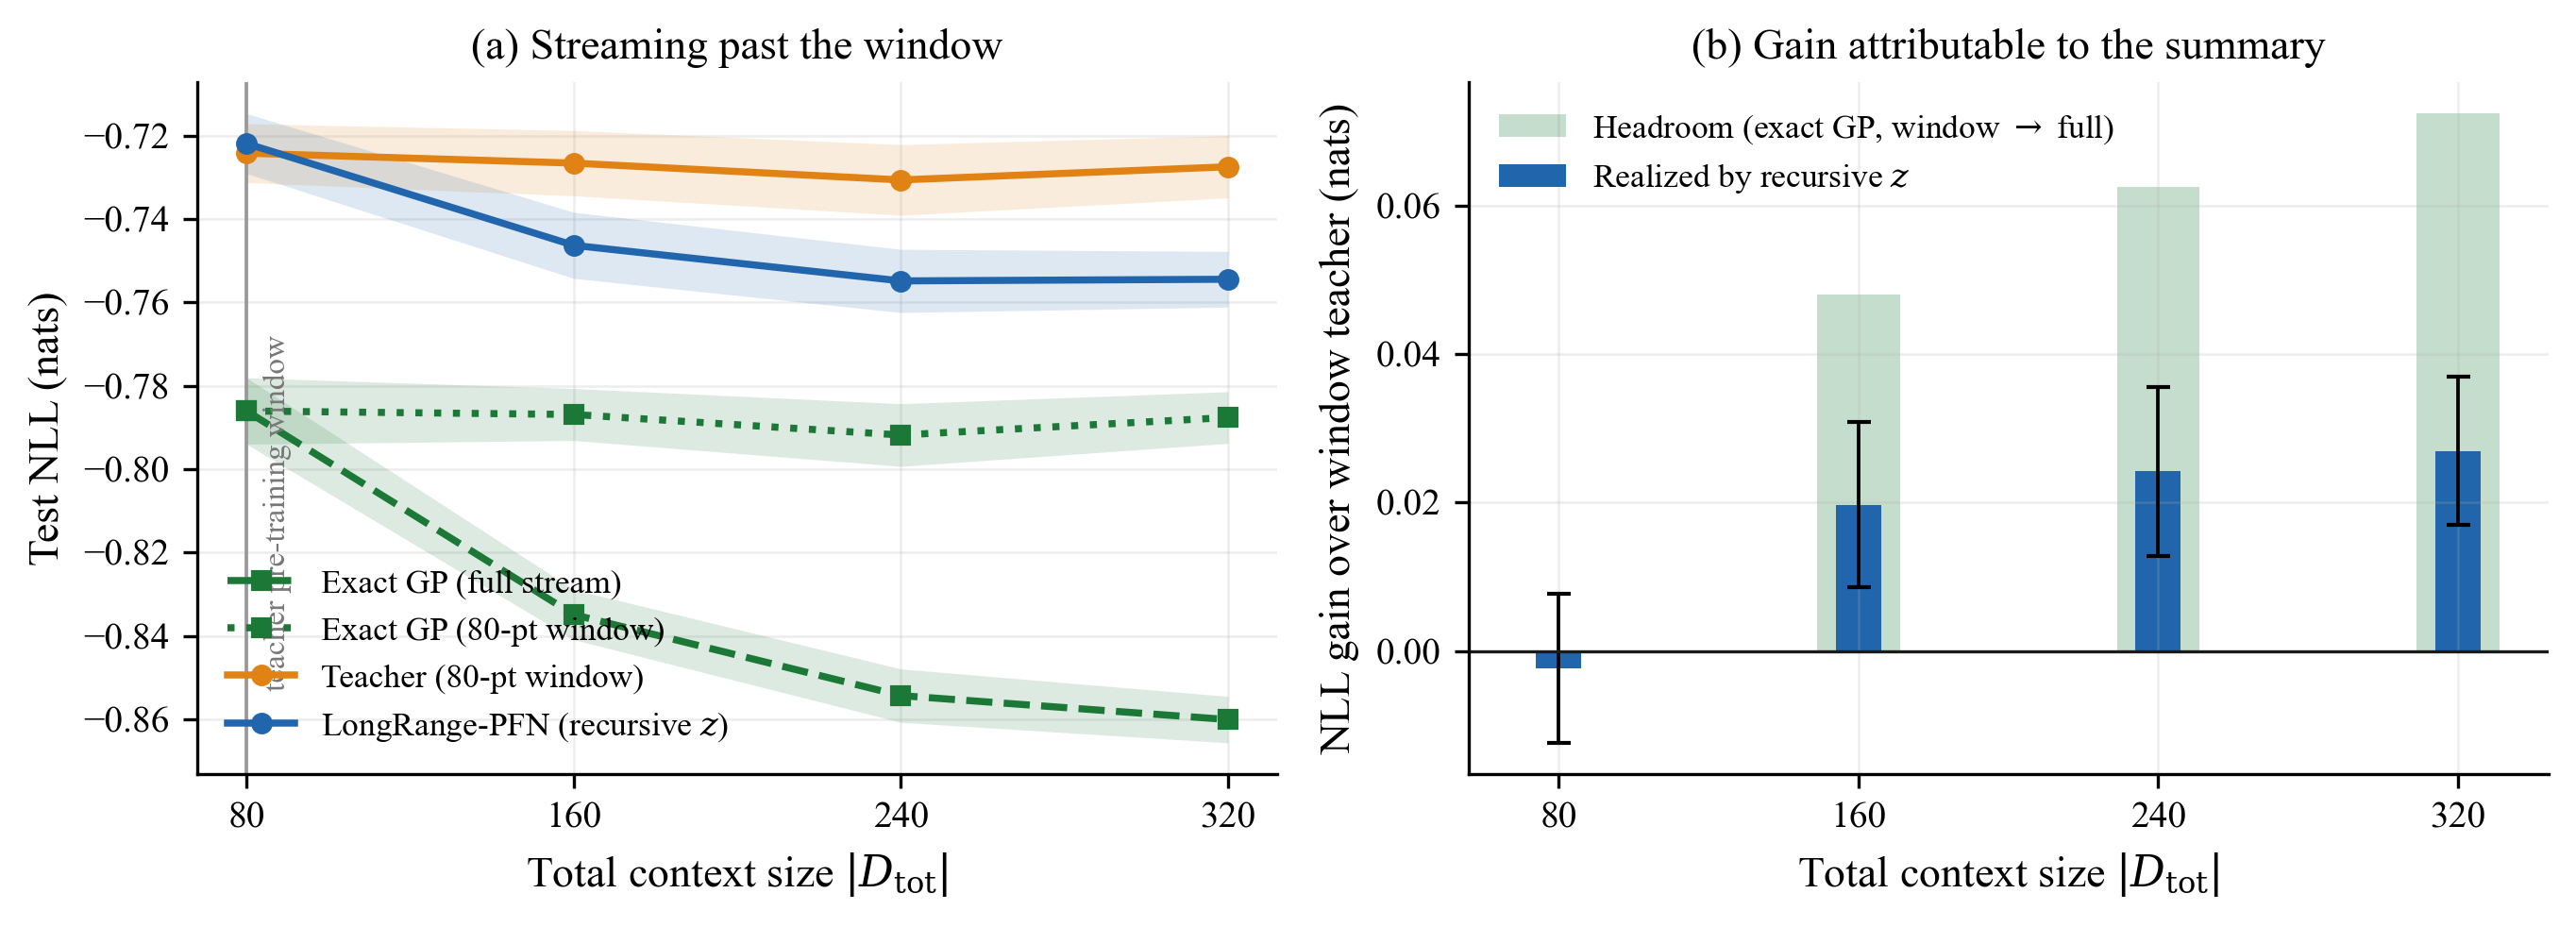
\includegraphics[width=\linewidth]{../results/beyond_window.png}
\caption{\textbf{Streaming beyond the pre-training window} (matched window
budgets, mean $\pm$ 95\% CI over $1{,}280$ data sets per point).
(a)~Test NLL vs.\ total context size: the window-limited teacher (orange) is
flat by construction, the exact GP on the full stream (green, dashed)
improves with evidence, and the recursive student (blue) tracks the teacher
at $|\Dtot|=80$ and then surpasses it as the stream grows. (b)~The gain
over the window teacher realized by the summary (blue bars) against the
headroom between the windowed and full exact posteriors (green bars); the
recursion recovers roughly a third of it.}
\label{fig:beyond}
\end{figure}

\begin{figure}[t]
\centering
\begin{minipage}[t]{0.48\linewidth}
\centering
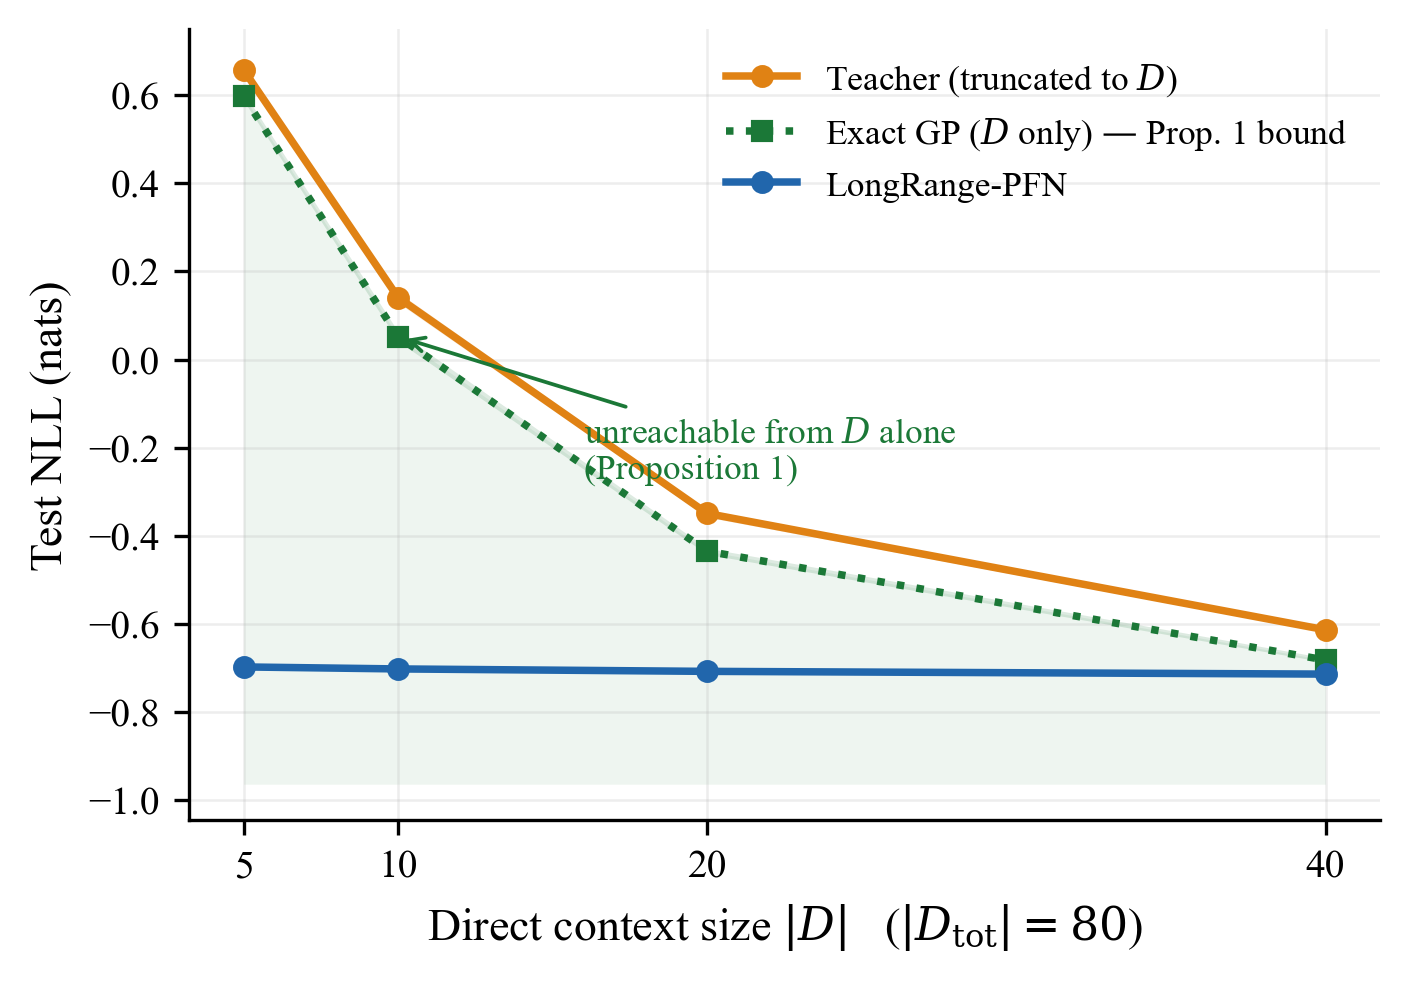
\includegraphics[width=\linewidth]{../results/certificate.png}
\caption{\textbf{The Proposition~\ref{prop:bound} certificate.} The exact GP
restricted to $\Dloc$ (green, dotted) lower-bounds the expected NLL of any
method that sees only $\Dloc$; the shaded region is unreachable without
outside information. The student (blue) sits inside it at every tested
$|\Dloc|$, close to the full-context optimum.}
\label{fig:certificate}
\end{minipage}\hfill
\begin{minipage}[t]{0.48\linewidth}
\centering
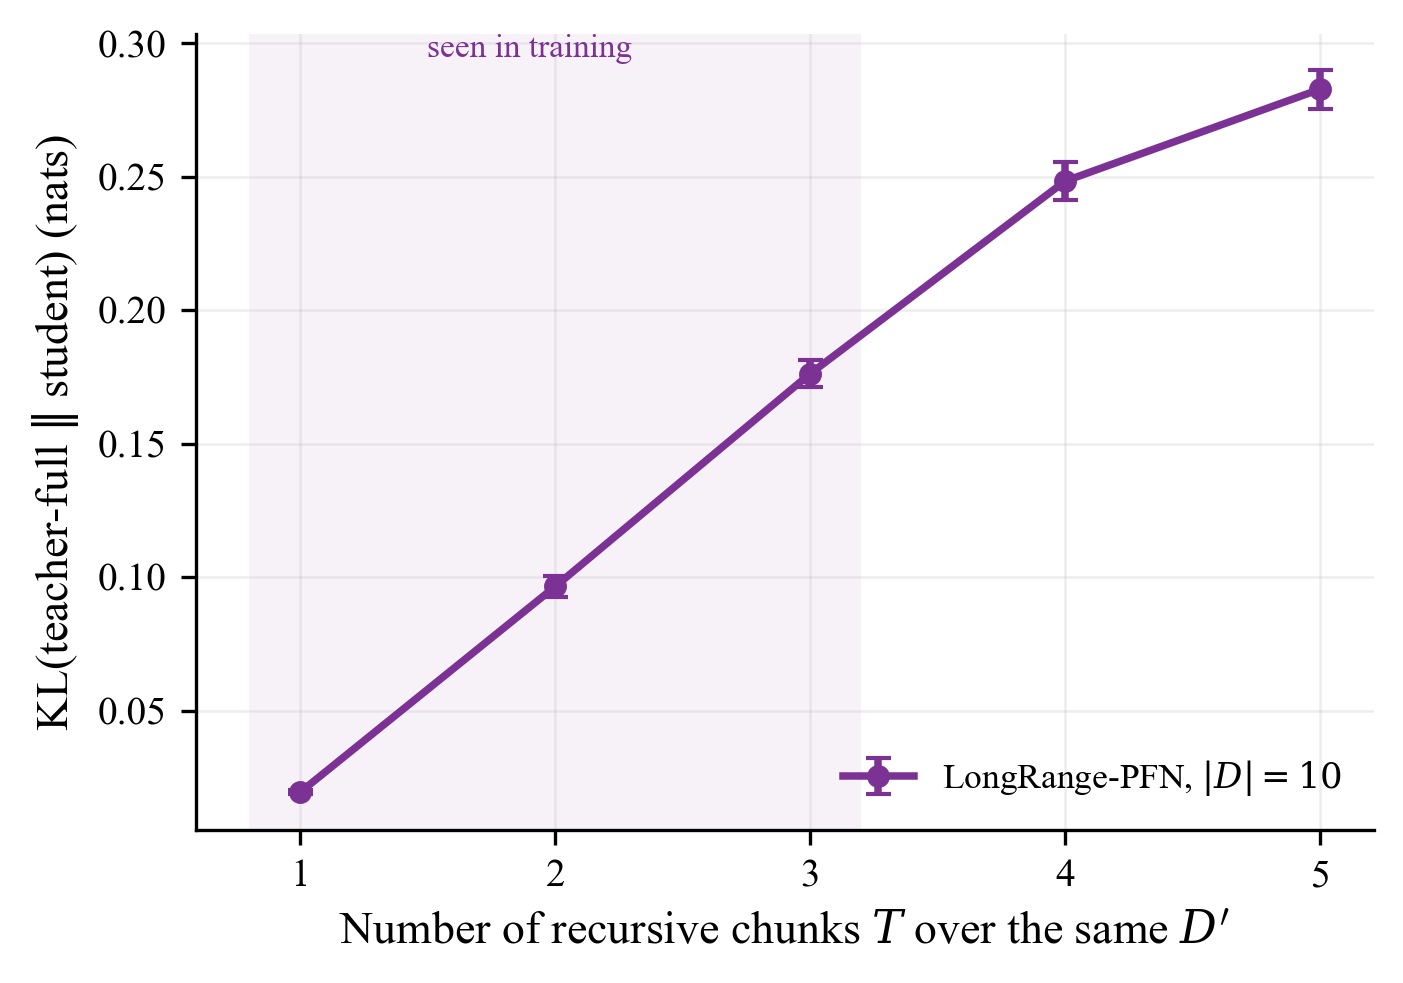
\includegraphics[width=\linewidth]{../results/chunks.png}
\caption{\textbf{Recursion cost.} KL to the full-context teacher when the
same $\Dfar$ ($|\Dfar|=70$, $|\Dloc|=10$) is folded in $T$ recursive
chunks. Cost rises from \chunkonekl{} nats at $T=1$ to \chunkfivekl{} nats
at $T=5$; $T \in \{4,5\}$ were never seen during distillation (shaded:
training range). The cost persists after adding multi-chunk regimes to the
model-selection criterion and fine-tuning, so it is not a selection
artifact; its near-linear growth in $T$ is consistent with error
compounding once per recursive step.}
\label{fig:chunks}
\end{minipage}
\end{figure}

\begin{figure}[t]
\centering
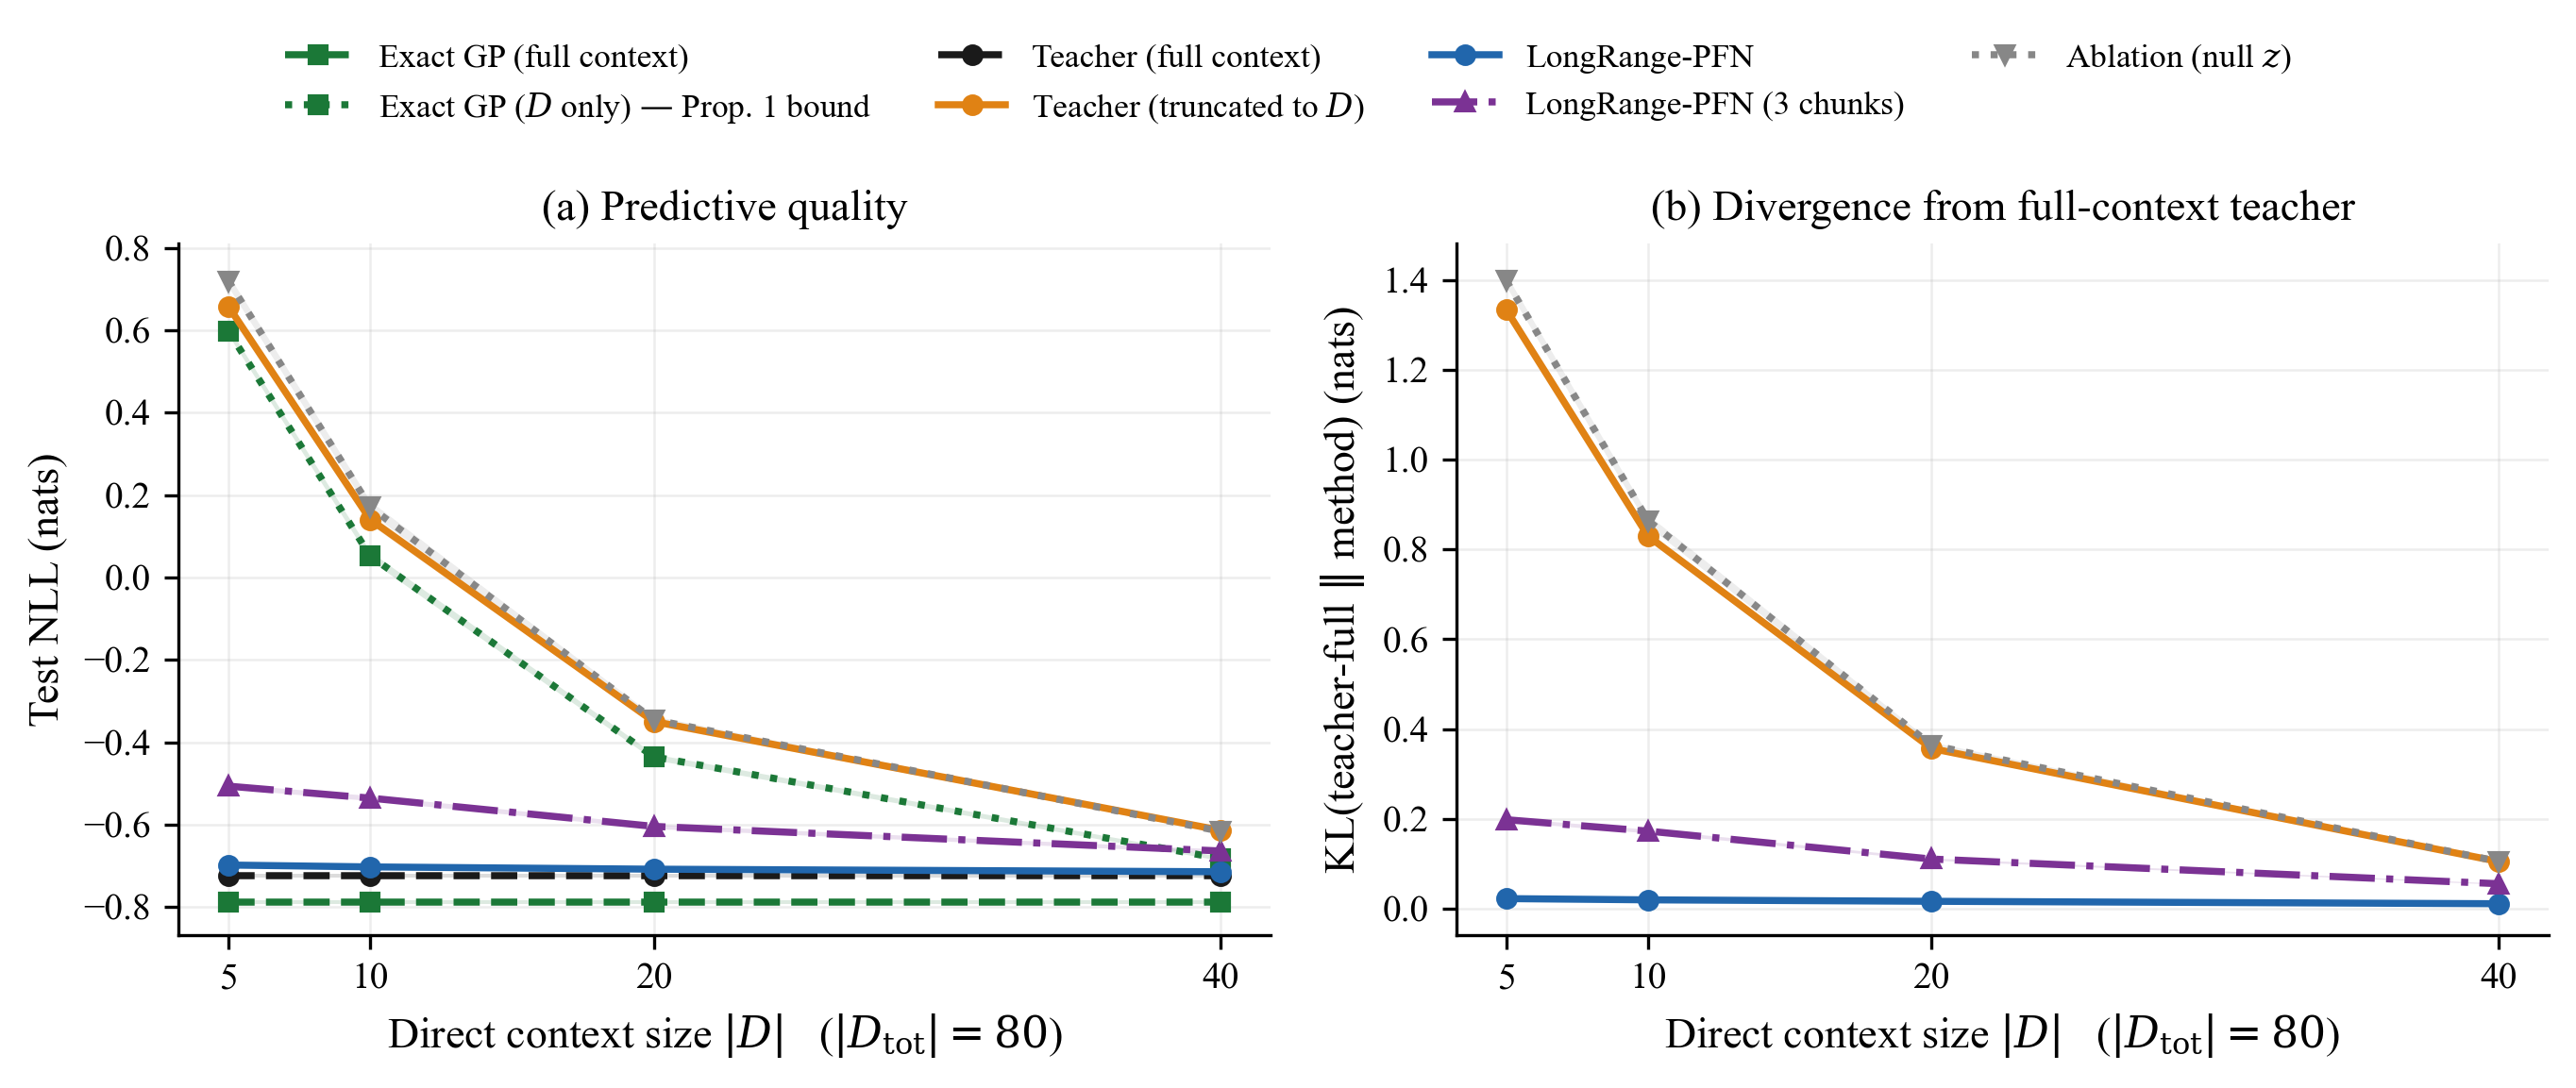
\includegraphics[width=\linewidth]{../results/sweep.png}
\caption{\textbf{Closing the truncation gap} (mean $\pm$ 95\% CI over
$3{,}200$ data sets). (a)~Test NLL vs.\ $|\Dloc|$: the single-shot latent
summary (blue) tracks the full-context reference (black, dashed) almost
exactly and stays below the exact-GP-on-$\Dloc$ bound (green, dotted); the
3-chunk variant (purple) trails both, consistent with
Figure~\ref{fig:chunks}. (b)~KL to the full-context teacher; the no-$z$
ablation (gray) tracks plain truncation.}
\label{fig:sweep}
\end{figure}

\begin{figure}[t]
\centering
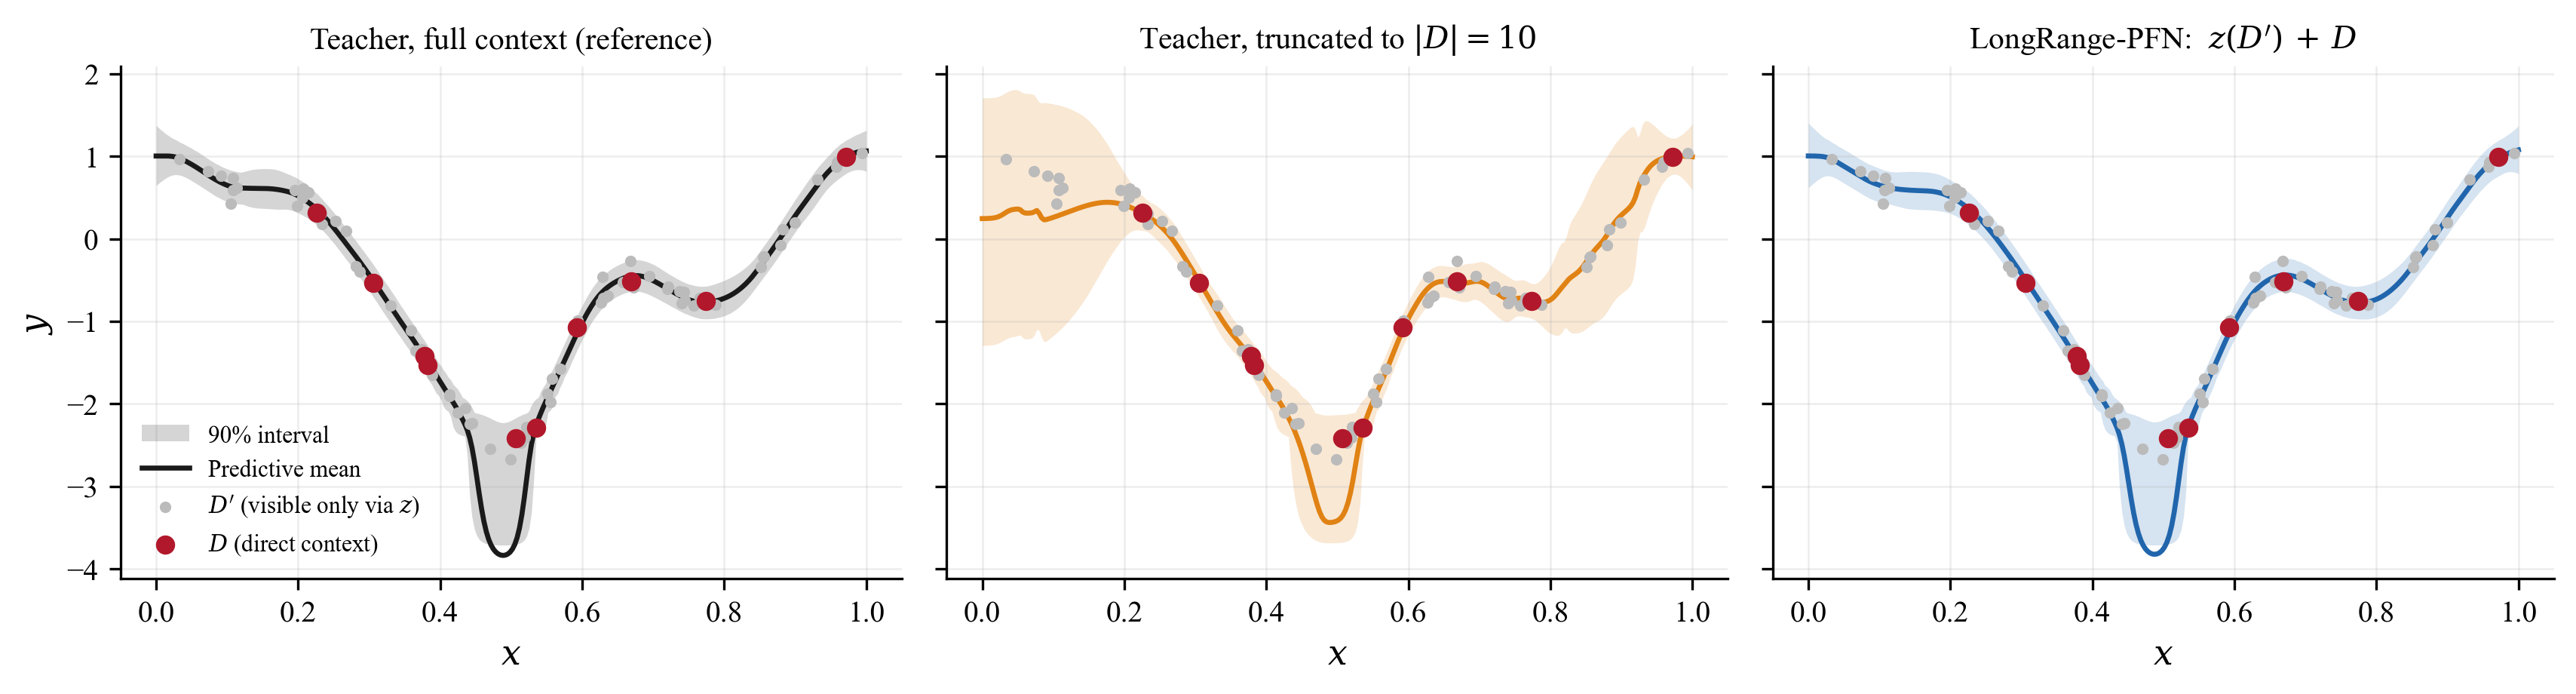
\includegraphics[width=\linewidth]{../results/qualitative.png}
\caption{\textbf{Qualitative behaviour} on one GP draw ($|\Dloc|=10$, red
points; $\Dfar$, gray points, visible to the student only through $z$).
Predictive mean and 90\% interval. The truncated PFN (middle) is
overdispersed away from $\Dloc$; LongRange-PFN (right) sharpens toward the
full-context predictive (left) using the latent summary alone.}
\label{fig:qual}
\end{figure}

\paragraph{Calibration and where the summary helps.} Since training uses a
forward KL, the student should preserve the teacher's uncertainty rather
than sharpen it away. Coverage of central predictive intervals at
$|\Dloc|=10$ confirms this: the student's reliability curve sits closer to
the diagonal than truncation (which under-covers) or the full-context
teacher (mildly conservative). Binning test points by distance to the
nearest point of $\Dloc$ shows the student's gain over truncation growing
with that distance and vanishing near $\Dloc$ (Figure~\ref{fig:diagnostics}),
the spatial signature of the certificate in Section~\ref{sec:certificate},
and it also shows how much of the full-context gain is still uncaptured far
from $\Dloc$. A linear probe of $z$ (Appendix~\ref{app:probe}) finds the full-context
predictive mean almost fully linearly decodable from $\mathrm{vec}(z)$
across the whole input domain (held-out $R^2 \approx 0.97$ at every grid
location), so $z$ encodes the function itself rather than memorizing
individual points.

\begin{figure}[t]
\centering
\begin{minipage}[t]{0.48\linewidth}
\centering
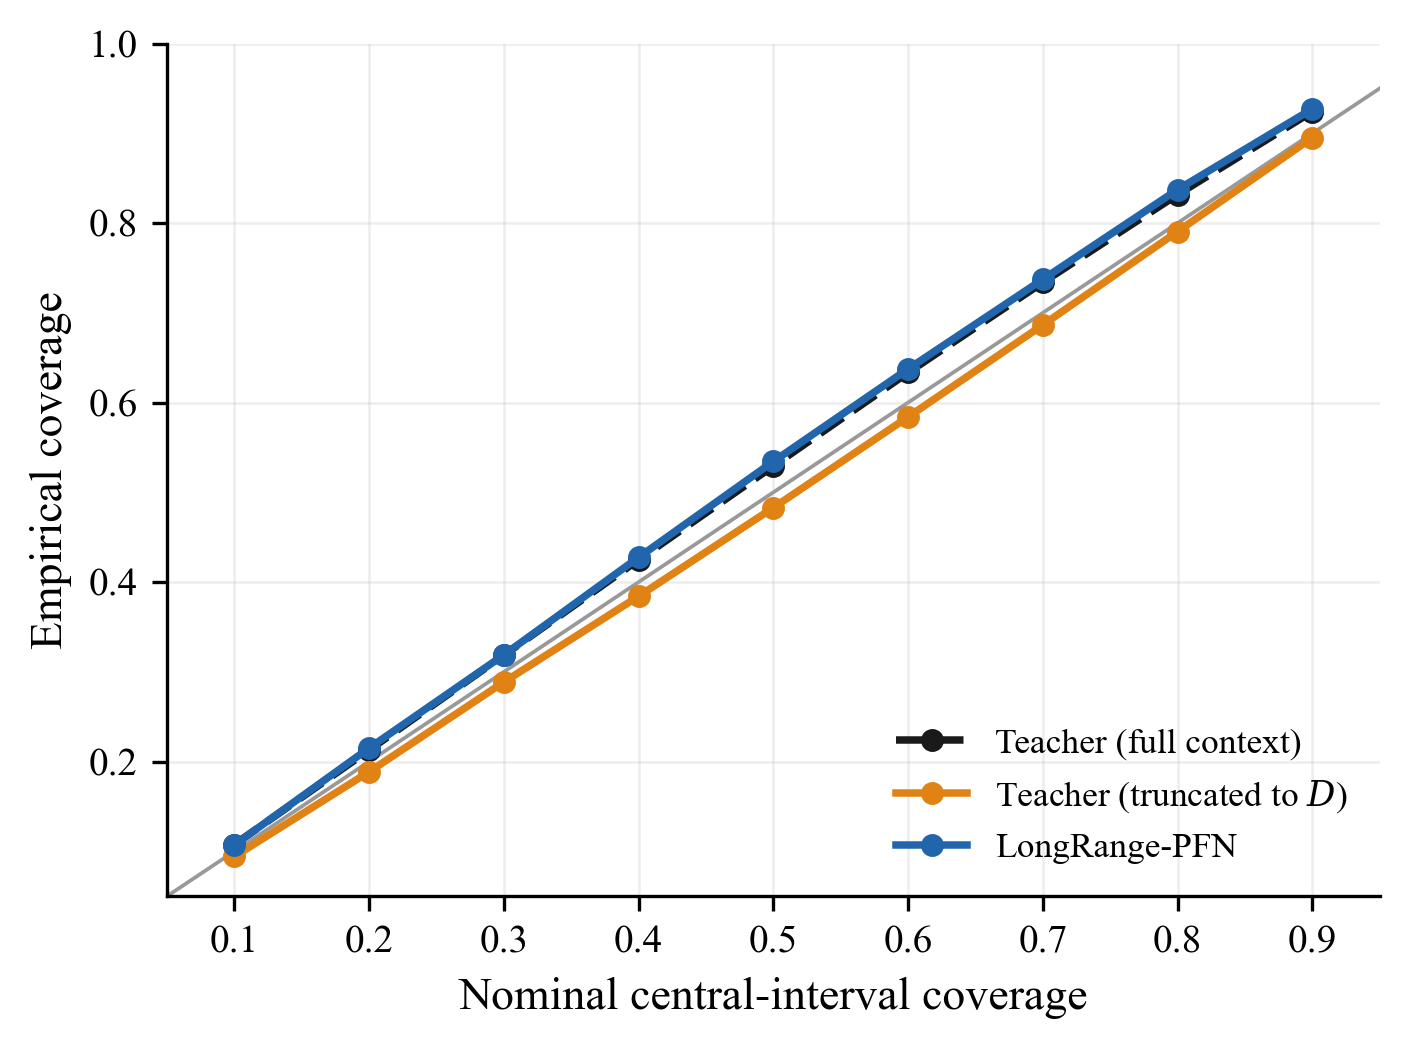
\includegraphics[width=\linewidth]{../results/calibration.png}
\end{minipage}\hfill
\begin{minipage}[t]{0.48\linewidth}
\centering
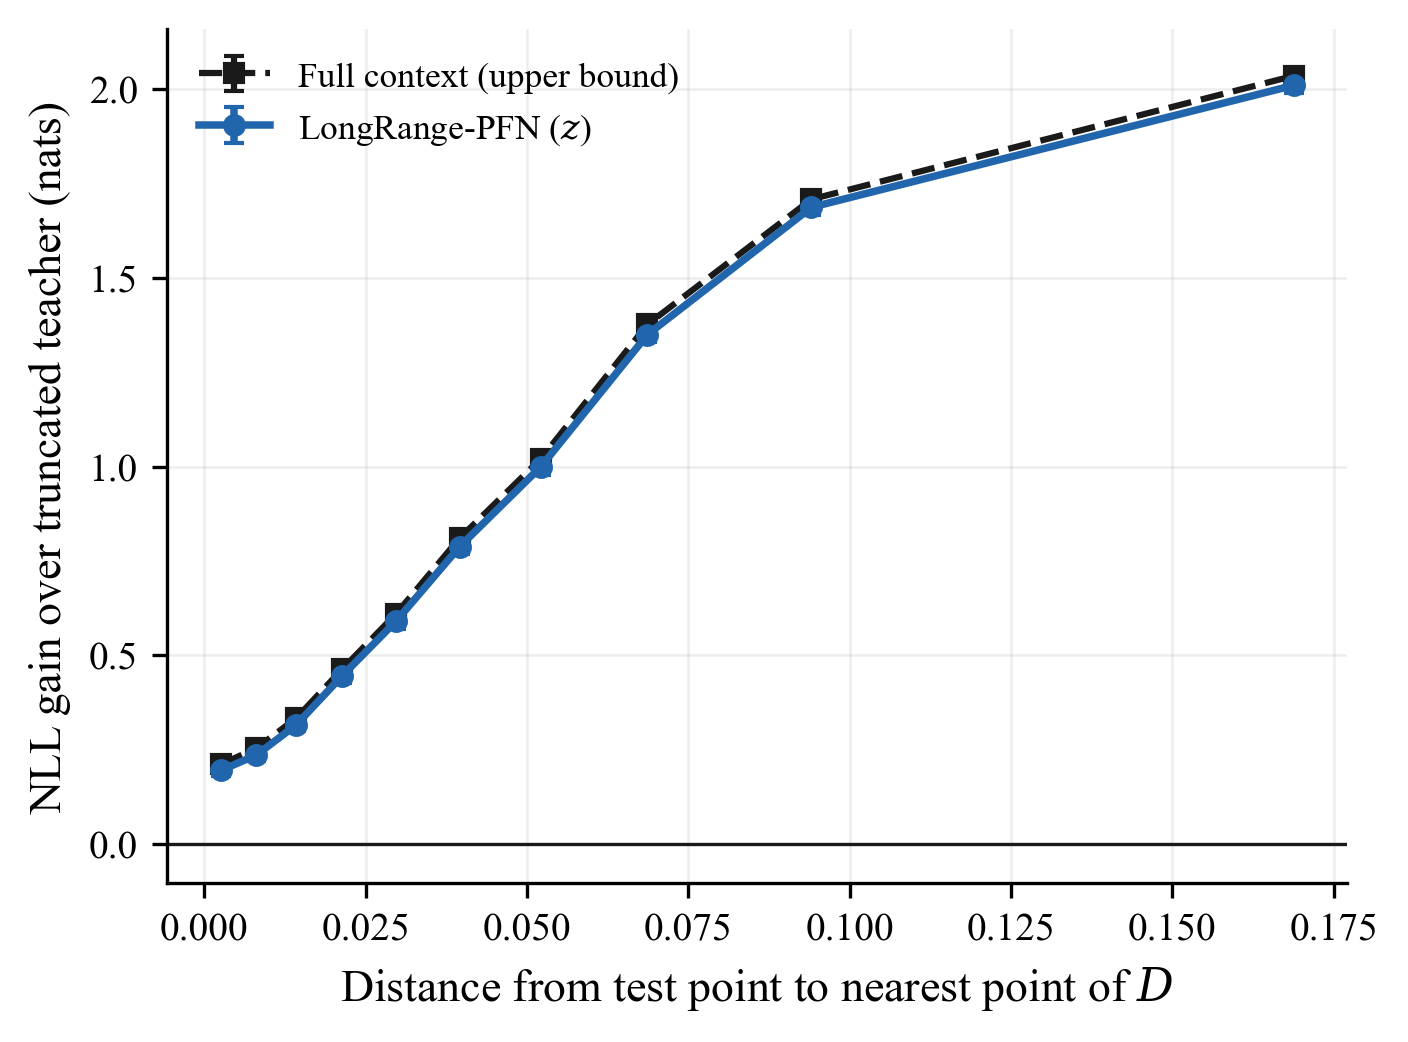
\includegraphics[width=\linewidth]{../results/where_it_helps.png}
\end{minipage}
\caption{\textbf{Diagnostics at $|\Dloc| = 10$.} Left: coverage of central
predictive intervals; the student (blue) sits closest to the diagonal,
truncation (orange) under-covers, and the full-context teacher (black,
dashed) is mildly conservative. Right: NLL gain over the truncated
teacher, binned by distance from the test point to the nearest point of
$\Dloc$ (mean $\pm$ 95\% CI); the gain grows with distance and stays below
the full-context ceiling (dashed).}
\label{fig:diagnostics}
\end{figure}

\section{Limitations}
\label{sec:limitations}

This is a proof of concept on a 1-d GP prior with a small teacher and
exchangeable contexts. Chunk boundaries do not matter here but would under
non-stationary or ordered data, where the recursion should be treated as a
proper filter. The summary size $k$ is an information bottleneck: a finite
$k$ cannot represent posteriors that concentrate on high-dimensional
structure, and we have not characterized the rate--distortion trade-off.
The distillation ceiling is the teacher's own quality within its window;
past that, the recursion is validated only empirically. The multi-chunk
cost (Figure~\ref{fig:chunks}) is a real limitation of the current
recursion: we ruled out the model-selection explanation by widening the
validation criterion and fine-tuning, and the near-linear growth in $T$
remained, so each recursive application of $\rep_\phi$ loses information
that more training does not recover. A more basic limit shows up
in Appendix~\ref{app:baselines}: a fitted classical GP or full-context
TabPFN still beat bounded-state inference here, simply because exact
inference on this prior is already cheap. A real advantage over such
methods needs a prior where exact inference is intractable and a teacher
closer to TabPFN's scale, plus query-aware summaries $z(x)$ and the
associativity regularizer from Section~\ref{sec:recursive}.

\section{Conclusion}

LongRange-PFN carries the evidence a PFN needs from out-of-window data in a
small set of latent tokens, trained only by distilling a frozen teacher's
predictive distribution. On GP priors, the summary provably carries
posterior information, it crosses the exact lower bound of
Proposition~\ref{prop:bound} at every context size tested, and the
recursive update handles streams four times the training window at
constant state while beating a strong recency baseline. Two gaps remain:
multi-chunk summarization lags single-shot quality because our validation
set never checked it, and bounded-state inference still trails classical
full-context methods on this easy prior. Both are concrete and measurable,
which is what the exact-posterior certificate is for.

\section*{Reproducibility statement}

All code (built on the official PFN repository), training scripts, seeds
and configurations, and the scripts that regenerate every number, table
and figure in this paper from \texttt{results/metrics.json} are in the
accompanying repository (\texttt{long\_range\_pfn/}, \texttt{paper/}).

\appendix

\section{Training curves}
\label{app:training}

\begin{figure}[H]
\centering
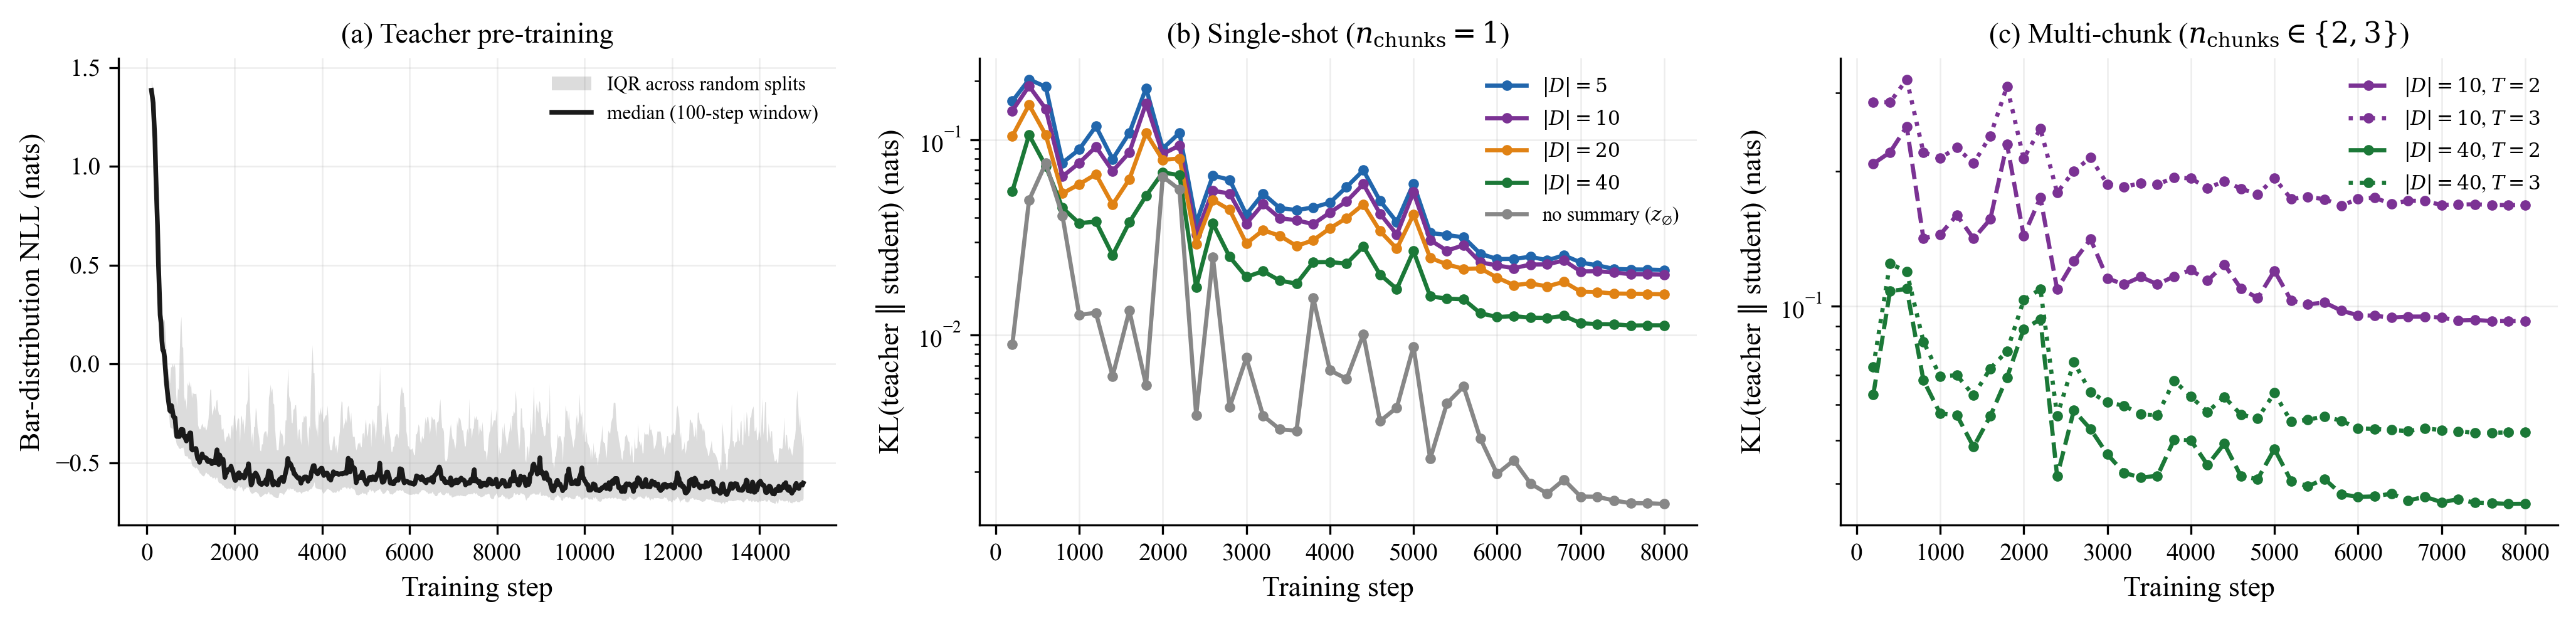
\includegraphics[width=\linewidth]{../results/training_curves.png}
\caption{\textbf{Optimization traces} behind the reported checkpoint.
(a)~Teacher pre-training: bar-distribution NLL on prior samples (rolling
median, solid; interquartile range, shaded). (b,~c)~The $8{,}000$-step
fine-tuning stage, tracked on the fixed, held-out validation set (resampled
once, same batches reused at every evaluation), one line per regime and
one panel per chunk count, a single pooled curve over raw training loss
would be unreadable, since regimes differ by two orders of magnitude in
scale. Single-shot regimes (b) refine at their floor; multi-chunk regimes
(c) improve modestly but stay well above it, the gap analyzed in
Section~\ref{sec:experiments}. The dynamics of the initial $15{,}000$-step
stage, including the phase transition, are in
Appendix~\ref{app:dynamics}.}
\label{fig:training}
\end{figure}

\section{Training dynamics: a phase transition, not grokking}
\label{app:dynamics}

Distillation does not improve smoothly. Figure~\ref{fig:dynamics}a shows
the fixed-validation KL of the initial $15{,}000$-step distillation
stage from
Section~\ref{sec:experiments}: every regime sits on a plateau for the
first $\sim\!6{,}000$ steps, drops by one to two orders of magnitude
between steps $6{,}000$ and $10{,}000$ ($11$--$49\times$ depending on
regime), then refines slowly. The transition is synchronized,
$|\Dloc| = 5$, $10$ and $20$ leave the plateau and reach the floor at the
same steps, which points to a single shared mechanism forming at once:
the circuit that routes information from the summary tokens into
predictions. This mirrors the abrupt formation of induction heads in
language models \citep{olsson2022induction}, where in-context ability
appears in a narrow window of training rather than accruing gradually. The
learning-rate schedule is a plain cosine with no restarts, so the window is
not a schedule artifact.

It is not grokking. Grokking \citep{power2022grokking} is delayed
generalization on a memorizable training set: training loss reaches its
floor early, held-out loss stays high, and the gap collapses much later.
Our distillation samples a fresh prior dataset at every step, so there is
no training set to memorize and the training loss is an unbiased estimate
of population loss. Figure~\ref{fig:dynamics}b confirms it: matched-regime
training KL and held-out validation KL move together throughout (log--log
correlation $0.98$), and validation is never worse than training. The jump
is a capability transition under online data, not a
memorization-to-generalization crossover.

This retroactively explains an earlier failure: a $5{,}000$-step run with
the same architecture stopped entirely on the plateau and closed only
$12\%$ of the truncation gap, against \shortclosepct{} after the
transition. Budgeting distillation past the transition matters more than
any other hyperparameter we tuned. Progress-measure analyses of the kind
used for induction heads \citep{nanda2023progress}, for instance,
tracking attention mass from test tokens to summary tokens over training,
are the natural tool for identifying what forms inside the window, and we
leave this to future work.

\begin{figure}[H]
\centering
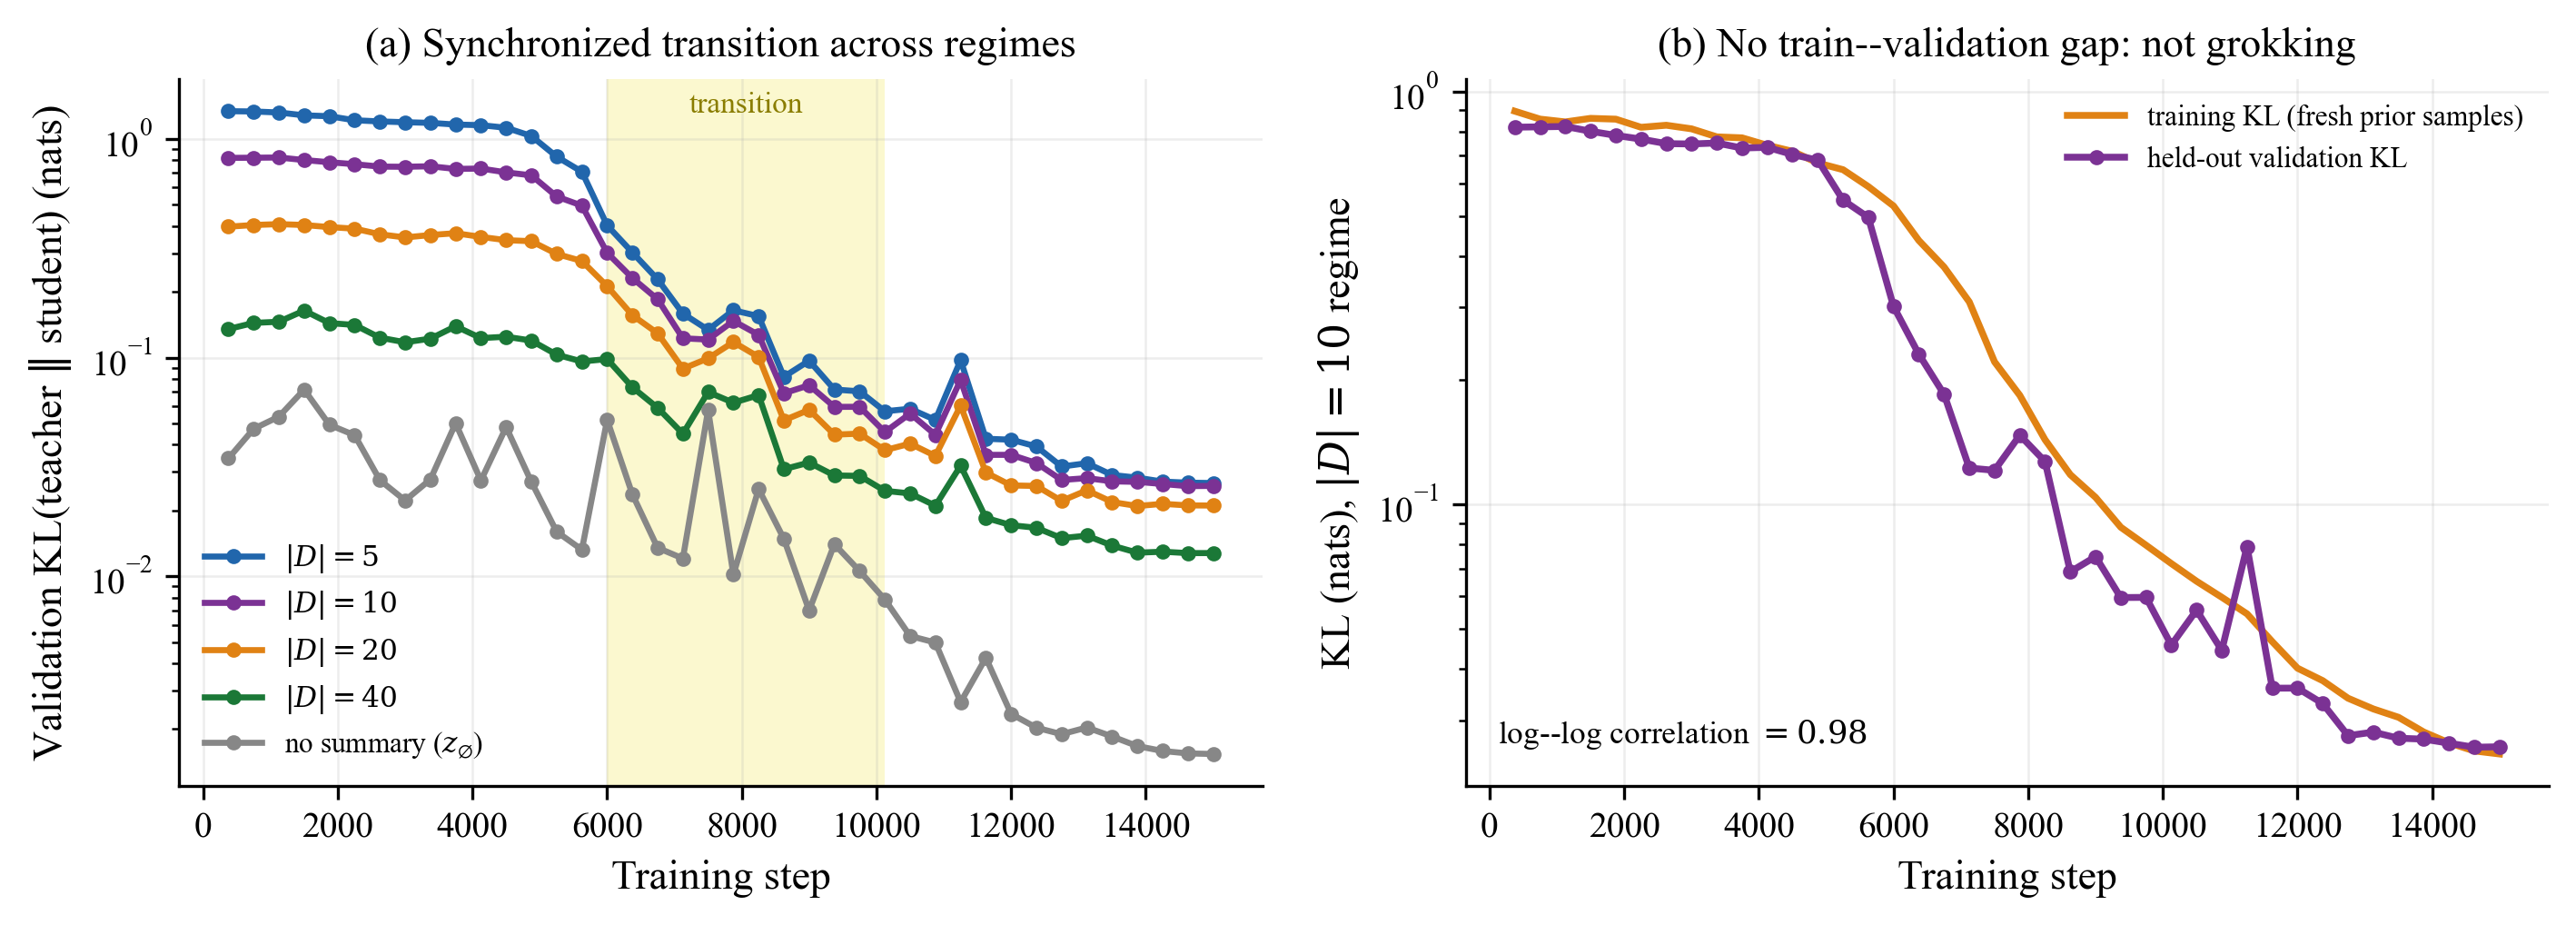
\includegraphics[width=\linewidth]{../results/dynamics.png}
\caption{\textbf{Training dynamics of distillation} ($15{,}000$-step run).
(a)~Held-out validation KL per regime: a long plateau, then a synchronized
$11$--$49\times$ drop between steps $6{,}000$ and $10{,}000$ (shaded), then
slow refinement. (b)~The grokking discriminator at $|\Dloc| = 10$:
training KL on fresh prior samples (matched-regime rolling median) against
held-out validation KL. The curves coincide (log--log correlation $0.98$);
the persistent train--validation gap that defines grokking never forms,
as expected with fresh data at every step.}
\label{fig:dynamics}
\end{figure}

\section{Defensive baselines at large context}
\label{app:baselines}

The main text compares against the teacher and the exact GP, asking
whether the summary preserves information that truncation destroys. A
harder question: why not just give all the data to a method with no window
at all? TabPFN, a Gaussian process, and a random forest have no $80$-point
limit, so here we give them the entire context, up to $8\times$ the
teacher's window, and check whether LongRange-PFN, a recent local window
plus an $O(k)$ recursive summary, still holds up.

Table~\ref{tab:baselines} covers $N \in \{80, 160, 320, 640\}$, using an
earlier teacher/student pair trained with a shorter schedule than
Section~\ref{sec:experiments}; the conclusion below does not depend on that
difference, since it follows from the prior being easy for a matched
kernel rather than from any specific checkpoint, but we flag the mismatch
and plan to refresh the table. The full-context baselines are TabPFN
\citep{hollmann2025tabpfn}, a scikit-learn GP with an RBF kernel fit per
dataset (unlike the oracle ``GP exact'', which uses the true generating
hyperparameters), kernel ridge regression, $k$-NN, and a random forest, all
given the full $N$ points; LongRange-PFN and the recency-window teacher see
only bounded state. We report NLL for the probabilistic methods and RMSE
for all.

A fitted RBF-kernel GP ends up close to the exact oracle here, which is
not surprising, the data come from an RBF GP, so a matched kernel is
close to optimal by construction. Full-context TabPFN is also strong. Both
beat the bounded-state methods in NLL by roughly $0.1$--$0.2$ nats. This is
an easy point-prediction task for a matched kernel: kernel ridge and the
fitted GP get the lowest RMSE, and only $k$-NN and the random forest are
clearly weak, so the setting was never going to show a predictive win over
classical methods. That is fine, because the contribution is not a better
predictor on GP data, where exact inference is already cheap, it is a
bounded-state mechanism for carrying evidence when the full context cannot
be stored and re-attended, the case Section~\ref{sec:experiments} argues
for. A real predictive win over strong full-data baselines would need a
prior where exact inference is intractable and a teacher closer to
TabPFN's scale.

\begin{table}[H]
\centering
\caption{Large-context defensive baselines over total context size $N$
(up to $8\times$ the teacher's window; $100$ datasets per cell, TabPFN on
its own smaller sample, noted in text). \emph{Full-context} baselines see
all $N$ points; \emph{bounded-state} methods (teacher-window, LongRange-PFN)
see only recent points plus, for LongRange-PFN, the $O(k)$ recursive
summary. NLL (nats) for probabilistic methods, RMSE for all; mean $\pm$
s.e.}
\label{tab:baselines}
\resizebox{\textwidth}{!}{\begin{tabular}{lcccc}
\toprule
\multicolumn{5}{c}{\emph{NLL (nats, lower is better)}}\\
\midrule
Method & $N=80$ & $N=160$ & $N=320$ & $N=640$\\
\midrule
Teacher (80-pt window) & -0.693\,{\scriptsize$\pm$0.016} & -0.682\,{\scriptsize$\pm$0.015} & -0.697\,{\scriptsize$\pm$0.014} & -0.716\,{\scriptsize$\pm$0.014}\\
\textbf{LongRange-PFN (bounded)} & -0.678\,{\scriptsize$\pm$0.016} & -0.662\,{\scriptsize$\pm$0.014} & -0.684\,{\scriptsize$\pm$0.014} & -0.702\,{\scriptsize$\pm$0.012}\\
GP exact (full, oracle) & -0.789\,{\scriptsize$\pm$0.012} & -0.824\,{\scriptsize$\pm$0.011} & -0.859\,{\scriptsize$\pm$0.011} & -0.893\,{\scriptsize$\pm$0.010}\\
TabPFN (full context) & -0.632\,{\scriptsize$\pm$0.024} & -0.723\,{\scriptsize$\pm$0.020} & -0.782\,{\scriptsize$\pm$0.020} & -0.756\,{\scriptsize$\pm$0.024}\\
GP-RBF fitted (full) & -0.771\,{\scriptsize$\pm$0.014} & -0.815\,{\scriptsize$\pm$0.011} & -0.856\,{\scriptsize$\pm$0.011} & -0.891\,{\scriptsize$\pm$0.011}\\
\midrule
\multicolumn{5}{c}{\emph{RMSE (lower is better)}}\\
\midrule
Method & $N=80$ & $N=160$ & $N=320$ & $N=640$\\
\midrule
Teacher (80-pt window) & 0.142\,{\scriptsize$\pm$0.008} & 0.154\,{\scriptsize$\pm$0.009} & 0.148\,{\scriptsize$\pm$0.009} & 0.140\,{\scriptsize$\pm$0.008}\\
\textbf{LongRange-PFN (bounded)} & 0.141\,{\scriptsize$\pm$0.008} & 0.153\,{\scriptsize$\pm$0.008} & 0.147\,{\scriptsize$\pm$0.009} & 0.139\,{\scriptsize$\pm$0.008}\\
GP exact (full, oracle) & -- & -- & -- & --\\
TabPFN (full context) & 0.120\,{\scriptsize$\pm$0.004} & 0.106\,{\scriptsize$\pm$0.002} & 0.103\,{\scriptsize$\pm$0.002} & 0.101\,{\scriptsize$\pm$0.002}\\
GP-RBF fitted (full) & 0.111\,{\scriptsize$\pm$0.002} & 0.106\,{\scriptsize$\pm$0.001} & 0.102\,{\scriptsize$\pm$0.001} & 0.099\,{\scriptsize$\pm$0.001}\\
Kernel ridge (full) & 0.110\,{\scriptsize$\pm$0.002} & 0.106\,{\scriptsize$\pm$0.001} & 0.102\,{\scriptsize$\pm$0.001} & 0.098\,{\scriptsize$\pm$0.001}\\
$k$-NN (full) & 0.164\,{\scriptsize$\pm$0.004} & 0.125\,{\scriptsize$\pm$0.002} & 0.113\,{\scriptsize$\pm$0.001} & 0.109\,{\scriptsize$\pm$0.001}\\
Random forest (full) & 0.142\,{\scriptsize$\pm$0.003} & 0.127\,{\scriptsize$\pm$0.002} & 0.123\,{\scriptsize$\pm$0.001} & 0.121\,{\scriptsize$\pm$0.001}\\
\bottomrule
\end{tabular}
}
\end{table}

\section{What does the summary encode?}
\label{app:probe}

\begin{figure}[H]
\centering
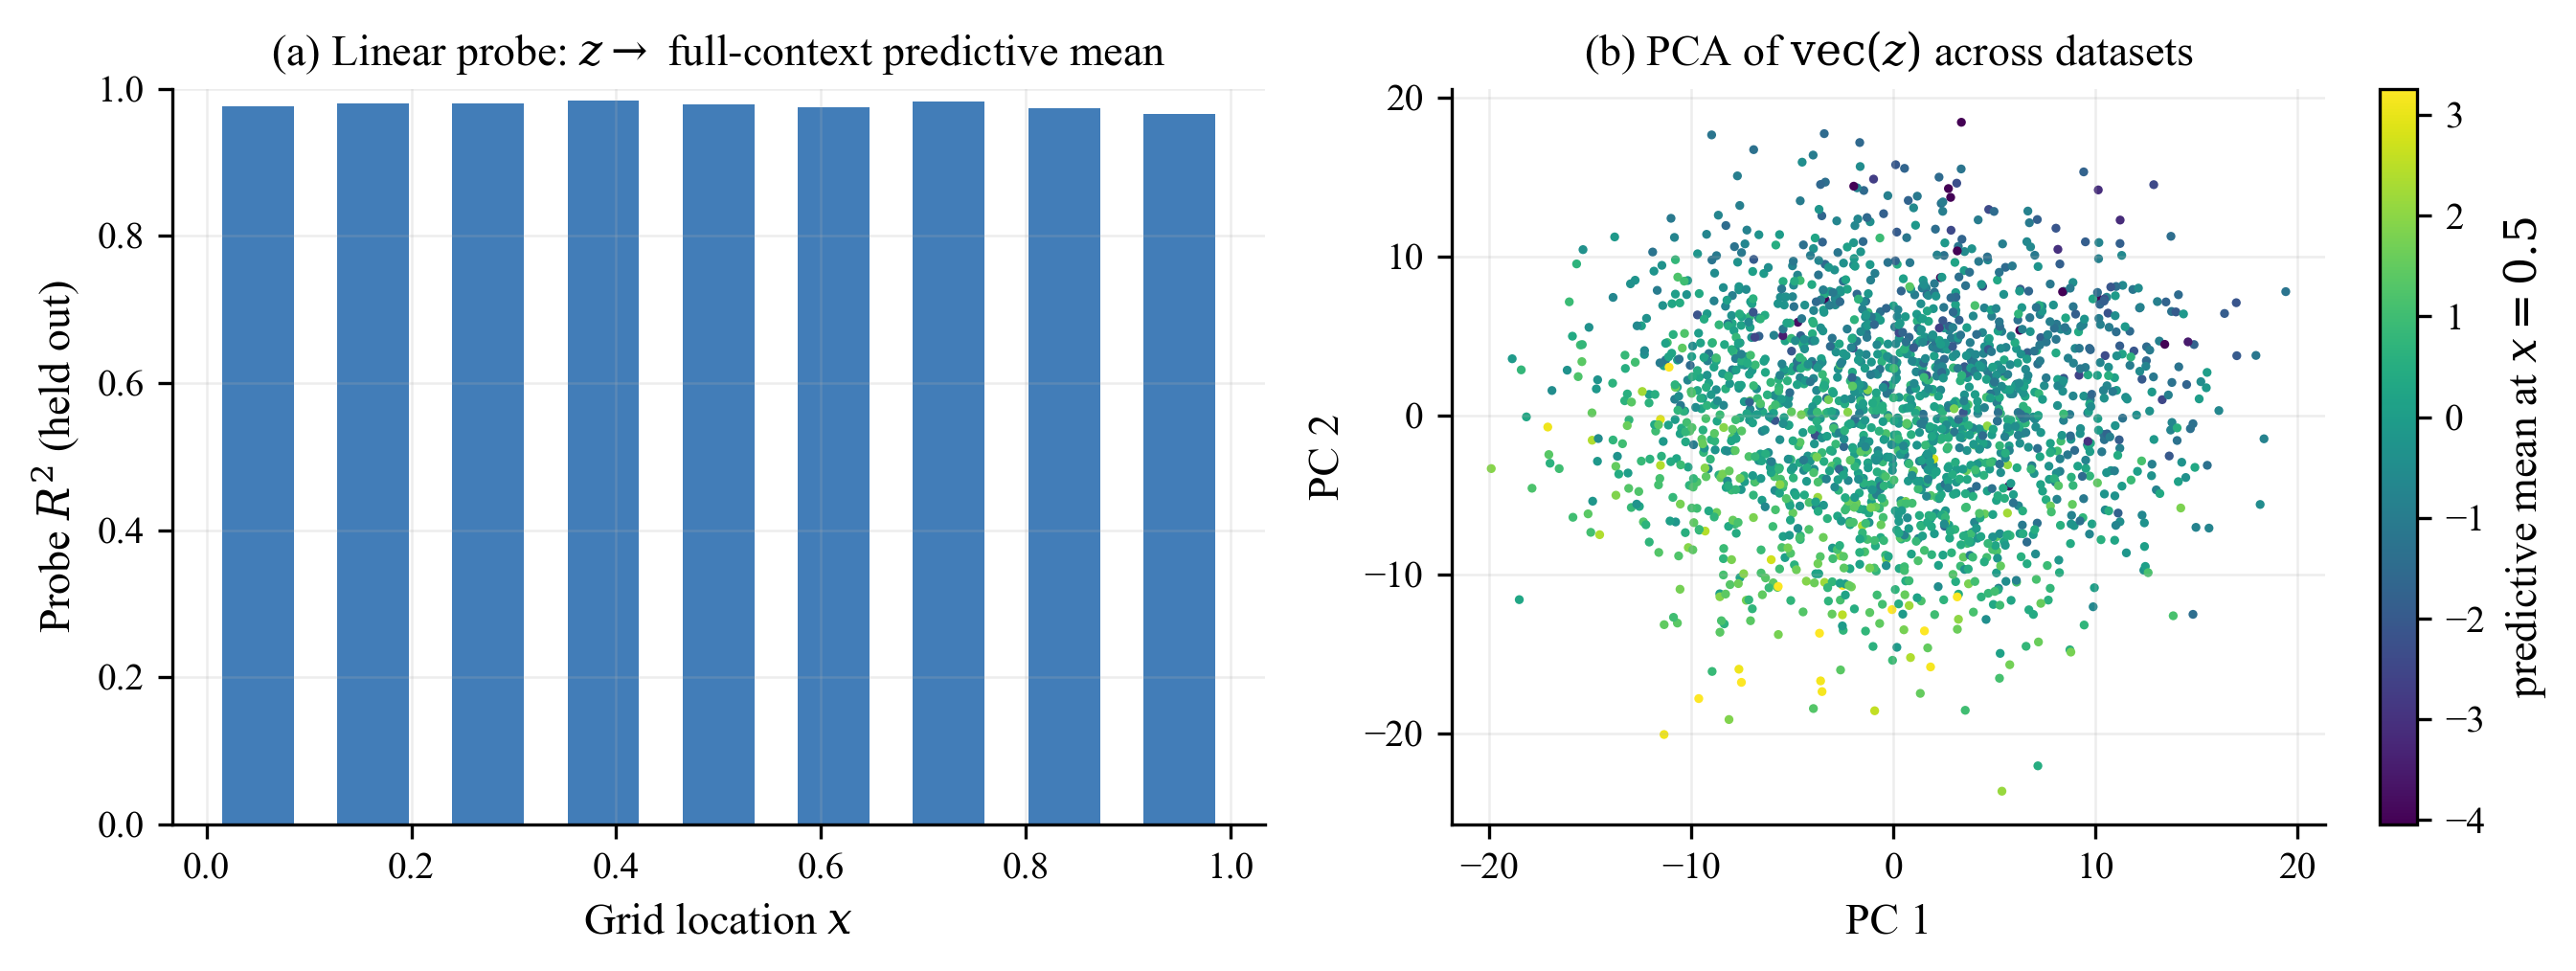
\includegraphics[width=\linewidth]{../results/latent_probe.png}
\caption{\textbf{Probing the summary space} ($z$ computed from all $80$
context points; $\approx 1{,}900$ held-out datasets). (a)~Held-out $R^2$ of
a ridge probe from $\mathrm{vec}(z)$ to the full-context teacher's
predictive mean at each grid location: after the phase transition of
Appendix~\ref{app:dynamics}, the function is almost fully linearly
decodable from the summary everywhere in the domain ($R^2 \approx 0.97$ at
every location; a pre-transition checkpoint reached only $0.3$--$0.9$).
(b)~First two principal components of $\mathrm{vec}(z)$, colored by the
predictive mean at $x=0.5$: the summary space is organized by function
value along a clear gradient.}
\label{fig:probe}
\end{figure}

\begin{thebibliography}{18}

\bibitem[M\"uller et al.(2022)]{muller2022pfn}
S.~M\"uller, N.~Hollmann, S.~Pineda-Arango, J.~Grabocka, F.~Hutter.
\newblock Transformers Can Do Bayesian Inference.
\newblock \emph{ICLR}, 2022.

\bibitem[Hollmann et al.(2023)]{hollmann2023tabpfn}
N.~Hollmann, S.~M\"uller, K.~Eggensperger, F.~Hutter.
\newblock TabPFN: A Transformer That Solves Small Tabular Classification
Problems in a Second.
\newblock \emph{ICLR}, 2023.

\bibitem[Hollmann et al.(2025)]{hollmann2025tabpfn}
N.~Hollmann, S.~M\"uller, L.~Purucker, A.~Krishnakumar, M.~K\"orfer,
S.~B.~Hoo, R.~T.~Schirrmeister, F.~Hutter.
\newblock Accurate predictions on small data with a tabular foundation
model.
\newblock \emph{Nature}, 637:319--326, 2025.

\bibitem[Feuer et al.(2024)]{feuer2024tunetables}
B.~Feuer, R.~T.~Schirrmeister, V.~Cherepanova, C.~Hegde, F.~Hutter,
M.~Goldblum, N.~Cohen, C.~White.
\newblock TuneTables: Context Optimization for Scalable Prior-Data Fitted
Networks.
\newblock \emph{NeurIPS}, 2024.

\bibitem[Ma et al.(2024)]{ma2024icd}
J.~Ma, V.~Thomas, G.~Yu, A.~Caterini.
\newblock In-Context Data Distillation with TabPFN.
\newblock \emph{arXiv:2402.06971}, 2024.

\bibitem[Thomas et al.(2024)]{thomas2024localpfn}
V.~Thomas, J.~Ma, R.~Hosseinzadeh, K.~Golestan, G.~Yu, M.~Volkovs,
A.~Caterini.
\newblock Retrieval \& Fine-Tuning for In-Context Tabular Models.
\newblock \emph{NeurIPS}, 2024.

\bibitem[Heredge et al.(2026)]{heredge2026crumb}
J.~Heredge, M.~J.~Villani, P.~Deshpande, A.~Seshadri, N.~Kumar.
\newblock CRUMB: Efficient Prior Fitted Network Inference via
Distributionally Matched Context Batching.
\newblock \emph{arXiv:2606.11473}, 2026.

\bibitem[Mu et al.(2023)]{mu2023gisting}
J.~Mu, X.~L.~Li, N.~Goodman.
\newblock Learning to Compress Prompts with Gist Tokens.
\newblock \emph{NeurIPS}, 2023.

\bibitem[Ge et al.(2024)]{ge2023icae}
T.~Ge, J.~Hu, L.~Wang, X.~Wang, S.-Q.~Chen, F.~Wei.
\newblock In-context Autoencoder for Context Compression in a Large
Language Model.
\newblock \emph{ICLR}, 2024.

\bibitem[Chevalier et al.(2023)]{chevalier2023autocompressors}
A.~Chevalier, A.~Wettig, A.~Ajith, D.~Chen.
\newblock Adapting Language Models to Compress Contexts.
\newblock \emph{EMNLP}, 2023.

\bibitem[Bulatov et al.(2022)]{bulatov2022rmt}
A.~Bulatov, Y.~Kuratov, M.~Burtsev.
\newblock Recurrent Memory Transformer.
\newblock \emph{NeurIPS}, 2022.

\bibitem[Garnelo et al.(2018)]{garnelo2018np}
M.~Garnelo, J.~Schwarz, D.~Rosenbaum, F.~Viola, D.~J.~Rezende,
S.~M.~A.~Eslami, Y.~W.~Teh.
\newblock Neural Processes.
\newblock \emph{ICML Workshop on Theoretical Foundations and Applications
of Deep Generative Models}, 2018.

\bibitem[Kim et al.(2019)]{kim2019anp}
H.~Kim, A.~Mnih, J.~Schwarz, M.~Garnelo, A.~Eslami, D.~Rosenbaum,
O.~Vinyals, Y.~W.~Teh.
\newblock Attentive Neural Processes.
\newblock \emph{ICLR}, 2019.

\bibitem[Chen et al.(2021)]{chen2021nass}
Y.~Chen, D.~Zhang, M.~U.~Gutmann, A.~Courville, Z.~Zhu.
\newblock Neural Approximate Sufficient Statistics for Implicit Models.
\newblock \emph{ICLR}, 2021.

\bibitem[Mittal et al.(2025)]{mittal2025amortized}
S.~Mittal, N.~L.~Bracher, G.~Lajoie, P.~J\"akel, S.~Bauer.
\newblock Amortized In-Context Bayesian Posterior Estimation.
\newblock \emph{arXiv:2502.06601}, 2025.

\bibitem[Power et al.(2022)]{power2022grokking}
A.~Power, Y.~Burda, H.~Edwards, I.~Babuschkin, V.~Misra.
\newblock Grokking: Generalization Beyond Overfitting on Small Algorithmic
Datasets.
\newblock \emph{arXiv:2201.02177}, 2022.

\bibitem[Olsson et al.(2022)]{olsson2022induction}
C.~Olsson, N.~Elhage, N.~Nanda, N.~Joseph, et al.
\newblock In-context Learning and Induction Heads.
\newblock \emph{Transformer Circuits Thread}, 2022.

\bibitem[Nanda et al.(2023)]{nanda2023progress}
N.~Nanda, L.~Chan, T.~Lieberum, J.~Smith, J.~Steinhardt.
\newblock Progress Measures for Grokking via Mechanistic Interpretability.
\newblock \emph{ICLR}, 2023.

\bibitem[Hinton et al.(2015)]{hinton2015distillation}
G.~Hinton, O.~Vinyals, J.~Dean.
\newblock Distilling the Knowledge in a Neural Network.
\newblock \emph{NeurIPS Deep Learning Workshop}, 2015.

\bibitem[Korattikara et al.(2015)]{korattikara2015darkknowledge}
A.~Korattikara, V.~Rathod, K.~Murphy, M.~Welling.
\newblock Bayesian Dark Knowledge.
\newblock \emph{NeurIPS}, 2015.

\bibitem[Malinin et al.(2020)]{malinin2020edd}
A.~Malinin, B.~Mlodozeniec, M.~Gales.
\newblock Ensemble Distribution Distillation.
\newblock \emph{ICLR}, 2020.

\bibitem[M\"uller et al.(2023)]{muller2023pfns4bo}
S.~M\"uller, M.~Feurer, N.~Hollmann, F.~Hutter.
\newblock PFNs4BO: In-Context Learning for Bayesian Optimization.
\newblock \emph{ICML}, 2023.

\end{thebibliography}

\end{document}
